\documentclass[UTF8,zihao=-4,fontset=windows]{ctexart}
\usepackage[a4paper,margin=2.25cm,headheight=15pt]{geometry}
\usepackage{graphicx,booktabs,tabularx,array,amsmath,fancyhdr,caption,hyperref,float,tikz,enumitem,listings,xcolor,tocloft,placeins,needspace}
\usetikzlibrary{arrows.meta,positioning}
\newcolumntype{Y}{>{\raggedright\arraybackslash}X}
\hypersetup{colorlinks=true,linkcolor=black,urlcolor=black,citecolor=black,pdftitle={自动驾驶技术结课报告},pdfauthor={杜承敖}}
\setlength{\parindent}{2em}\setlength{\parskip}{0.24em}\setlength{\emergencystretch}{3em}
\renewcommand{\arraystretch}{1.24}\DeclareCaptionLabelSeparator{cncolon}{：}\captionsetup{font=small,labelfont=bf,labelsep=cncolon}
\lstset{basicstyle=\ttfamily\fontsize{9.5}{12}\selectfont,breaklines=true,frame=single,columns=fullflexible,keepspaces=true,showstringspaces=false,backgroundcolor=\color{gray!4},rulecolor=\color{gray!50},captionpos=b,aboveskip=9pt,belowskip=9pt}
\renewcommand{\lstlistingname}{代码清单}
\setcounter{secnumdepth}{3}\setcounter{tocdepth}{3}
\renewcommand{\thesection}{第\chinese{section}题}
\renewcommand{\thesubsection}{\arabic{section}.\arabic{subsection}}
\renewcommand{\thesubsubsection}{\thesubsection.\arabic{subsubsection}}
\setlength{\cftsecnumwidth}{4.1em}\setlength{\cftsubsecindent}{1.5em}\setlength{\cftsubsecnumwidth}{2.7em}\setlength{\cftsubsubsecindent}{4.2em}\setlength{\cftsubsubsecnumwidth}{3.6em}
\renewcommand{\cftsubsubsecfont}{\small}\renewcommand{\cftsubsubsecpagefont}{\small}
\renewcommand{\cfttoctitlefont}{\hfill\Large\bfseries\heiti}
\renewcommand{\cftaftertoctitle}{\hfill}
\ctexset{section={format=\Large\bfseries\heiti,beforeskip=1.1em,afterskip=.6em},subsection={format=\large\bfseries\heiti,beforeskip=1em,afterskip=.5em},subsubsection={format=\normalsize\bfseries\heiti,beforeskip=.8em,afterskip=.35em}}
\pagestyle{fancy}\fancyhf{}\fancyhead[L]{\small 自动驾驶技术结课报告}\fancyhead[R]{\small 系统组成 感知实践 规划决策}\fancyfoot[C]{\thepage}
\widowpenalty=10000\clubpenalty=10000
\raggedbottom
\setlength{\intextsep}{10pt plus 2pt minus 2pt}
\makeatletter
\DeclareRobustCommand{\figcite}[1]{%
  \begingroup
  \let\@cite\@firstoftwo
  \raisebox{.95ex}{\scriptsize\cite{#1}}%
  \endgroup
}
\makeatother
\newcommand{\paperfig}[6]{\begin{figure}[H]\centering\includegraphics[width=#2\textwidth,height=#3cm,keepaspectratio]{assets/papers/#1.png}\caption{#4\figcite{#5}}\label{#6}\end{figure}}
\begin{document}
\begin{titlepage}\centering\vspace*{1.8cm}
{\zihao{1}\heiti\bfseries 自动驾驶技术结课报告\par}\vspace{1.0cm}
{\zihao{3}\heiti 系统组成 感知实践与规划决策\par}\vspace{.4cm}
{\zihao{4}结合课程实验与实际智驾使用的分析\par}\vfill
{\zihao{4}\begin{tabular}{rl}姓名：&杜承敖\\[.6em]学号：&2024302112019\\[.6em]专业：&计算机科学与技术（雷军班）\\[.6em]课程：&自动驾驶技术\end{tabular}\par}\vfill
{\zihao{4}武汉大学\\[.4em]2026 年 11 月\par}\end{titlepage}
\pagenumbering{Roman}\tableofcontents\clearpage\pagenumbering{arabic}
\section*{摘要}
本报告按结题要求的三道题、十一个小问组织，结合四次课程实验及我的智驾使用观察，分析自动驾驶的系统结构、感知算法和规划决策。三次感知实践分别涉及图像二维检测、多相机三维检测和激光雷达三维检测，实验对比重点是输入、预训练、数据规模、任务和评价口径如何影响结果。行为克隆实践展示了图像到转向的训练过程，但尚无模拟器闭环结果。

我的使用感受是，基础路段驾驶已经稳定，但修路、检查配合和防御性预判仍暴露出不足。报告据此将讨论延伸到临时道路结构、人员指令、遮挡风险及交互僵局，并结合近期研究进一步分析时空占用、视觉语言动作、世界模型、闭环强化学习与生成式数据。核心认识是，识别对象、理解任务、生成动作与车辆正确执行，需要分别检查；常规道路的平均表现不足以说明长尾场景处理能力。

\noindent\textbf{关键词：}自动驾驶；nuScenes；环境感知；端到端驾驶；长尾场景；防御性驾驶

\noindent\textbf{材料说明：}实验数值和实验图片依据四次课程报告与保存结果；个人观察仅限本人所述使用体会，延伸案例及改进实验均作为分析方案。论文检索截至 2026 年 11 月 16 日，预印本按相应版本引用，论文配图以图注末尾的上标数字对应参考文献。
\section{自动驾驶系统组成与关键技术分析}
\FloatBarrier
\subsection{自动驾驶系统主要由哪些部分组成及其功能}
\subsubsection{主要模块与输入输出}
我把模块化自动驾驶理解为一个不断更新的闭环：系统先估计“周围是什么、自己在哪里”，再判断“接下来可能发生什么、应该怎样行驶”，最后把计划变成车辆动作。传感器层采集图像、激光雷达（Light Detection and Ranging，LiDAR）点云、毫米波雷达回波，以及全球导航卫星系统（Global Navigation Satellite System，GNSS）和惯性测量单元（Inertial Measurement Unit，IMU）等信息，并完成时间同步和标定；环境感知输出障碍物、车道、交通信号和可行驶区域；定位与地图提供自车位姿、道路结构及导航参考。行为预测估计其他交通参与者的未来运动，行为决策选择跟车、让行、停车或变道，轨迹规划求解可执行的时空轨迹，控制器驱动转向、制动和动力系统。

这些模块的输出应当同时包含时间和可信程度。一个“前方有行人”的标签还不够，规划需要其位置、速度、可能横穿的范围，以及这些估计有多大不确定性。系统还需要健康监测、数据记录和降级处理：传感器中断、定位退化或执行器未按指令动作，都应进入闭环检查。
\subsubsection{整体架构与模块之间的联系}
\begin{figure}[H]\centering
\begin{tikzpicture}[b/.style={draw,rounded corners,align=center,text width=30mm,minimum height=17mm,font=\small},a/.style={-{Stealth},thick},aux/.style={-{Stealth},thin}]
\draw[dashed,rounded corners,gray] (-7.45,1.30) rectangle (7.45,-3.85);
\node[fill=white,font=\small] at (0,1.30) {安全监测与降级覆盖输入、估计、决策、规划和执行};
\node[b](s) at (-5.55,0){多传感器输入\\Camera LiDAR\\Radar GNSS IMU};
\node[b](p) at (-1.85,0){环境感知\\检测 跟踪\\车道及场景识别};
\node[b](d) at (1.85,0){行为预测与决策\\运动预测 跟车\\变道 让行 停车};
\node[b](t) at (5.55,0){轨迹规划\\满足安全约束的\\时空轨迹};
\node[b](l) at (-1.85,-2.85){融合定位与地图\\自车位姿 导航\\道路及通行约束};
\node[b](f) at (1.85,-2.85){车辆状态反馈\\速度 转角\\执行误差};
\node[b](c) at (5.55,-2.85){车辆控制与执行\\轨迹跟踪\\转向 加速 制动};
\draw[a](s)--(p);\draw[a](p)--(d);\draw[a](d)--(t);\draw[a](t)--(c);
\draw[a](c)--(f);\draw[a](f)--(l);\draw[a](l)--node[left,font=\scriptsize]{位姿辅助}(p);
\draw[aux](s.south)--(-5.55,-2.85)--node[above,font=\scriptsize]{定位量测}(l.west);
\draw[aux](l.north east)--(-.1,-1.55)--node[above,font=\scriptsize]{导航与道路约束}(3.0,-1.55)--(t.south west);
\end{tikzpicture}
\caption{模块化自动驾驶系统架构。规划与控制独立；定位与地图辅助感知和规划，车辆状态进入下一轮更新。虚线边框表示安全监测对全流程的约束。}\label{fig:system}\end{figure}
图\ref{fig:system}中的箭头不仅传递目标框，还传递道路约束和车辆状态。例如定位使感知目标能与地图对齐，预测结果改变轨迹规划的安全空间，控制误差又影响下一次规划的初始条件。由此看，单模块准确率提高未必带来同等幅度的驾驶改进：若决策仍把检查点当作普通障碍物，感知框更准也可能只让绕行更顺畅。

感知、预测与规划可以围绕最终驾驶目标进行联合设计。我认为，模块划分有助于明确各部分的责任，系统评价还需要检验最终驾驶行为。课程前三次感知实验训练的检测器只覆盖其中一部分，第四次转向回归实验也不能替代完整闭环。

\FloatBarrier
\subsection{常用传感器及摄像头激光雷达毫米波雷达的特点和应用}
\subsubsection{三类环境传感器的比较}
\begin{table}[H]\centering\small\caption{主要传感器的特点与典型用途}
\begin{tabularx}{\textwidth}{lXXX}\toprule
传感器 & 优势 & 局限 & 典型应用\\\midrule
摄像头 & 纹理和颜色丰富，适于识别信号灯、标志和类别 & 光照、眩光、遮挡影响明显，单目深度存在歧义 & 车道线、交通标识、二维及多视角三维检测\\
激光雷达 & 直接获得稀疏三维距离与几何结构，利于测距 & 远处点稀疏；雨雾和遮挡影响回波，成本与算力需权衡 & 三维障碍物检测、定位与建图\\
毫米波雷达 & 测距及径向速度能力较强，对部分恶劣天气相对稳健 & 角分辨率和语义信息有限，存在虚警和多径 & 跟车测速、前向碰撞预警、辅助融合\\
其他 & GNSS、IMU、轮速计提供全球位置和短时运动信息 & GNSS 遮挡或多路径、惯性漂移及轮胎打滑 & 融合定位和状态估计\\\bottomrule\end{tabularx}\end{table}
\subsubsection{定位传感器与融合条件}
GNSS 提供全球位置参考，IMU 描述角速度和加速度，轮速计补充短时运动估计。它们与视觉或 LiDAR 里程计互补，但城市峡谷、隧道和打滑会使单一来源退化。融合应处理时间同步、坐标变换和量测不确定性，而不是把多个结果简单相加。

对于修路和检查点，我认为几何和语义尤其需要共同工作：LiDAR 可以指出锥桶、护栏和人的空间位置；相机能够提供标志文字、手势和灯光线索；毫米波雷达可补充周围车辆的径向速度。即使空间上存在空隙，也需要进一步确认那是被允许通行的路径。传感器选择因此取决于任务，不能用一次 mini 实验的检测分数 排出普遍优劣。

\FloatBarrier
\subsection{实际场景中从感知定位到规划控制的全过程}
\subsubsection{常规城市路口的完整闭环}
车辆按导航路线接近路口时，融合定位给出所在车道和距路口的位置；感知识别信号灯、斑马线及车辆行人，跟踪模块估计其运动。预测模块保留行人继续等待或横穿等可能性，决策模块选择减速、让行或通行，规划模块生成满足空间、速度和车辆运动约束的轨迹。控制器执行并用真实车速和转向反馈修正；环境变化后，整个过程重新计算。每一轮都必须在可接受的延迟内完成。
\subsubsection{修路与检查点为何要求不同决策}
结合我的智驾使用观察，基础路段的跟车和行驶已经比较稳定，但临时施工和酒驾检查仍容易暴露问题。施工可能使旧车道线通向封闭区域，需要根据现场锥桶、指示牌和人员活动重建可通行通道；遇到检查点时，则可能需要在被引导的位置停车等待。两种场景都能出现锥桶和人员，却不能共用“看到障碍就绕开”的行为。

从模块角度分析，施工首先挑战局部道路结构与地图的一致性；检查点更突出场景目的和人员指令理解。若系统已经知道前方有障碍，却仍试图绕过检查区域，问题可能出在场景理解或行为决策，也可能是相关证据未充分影响轨迹生成，仅凭一次外部观察无法确定具体内部故障。
\begin{table}[H]\centering\small\caption{外观相似的道路情境需要不同的行为解释}
\begin{tabularx}{\textwidth}{p{2.2cm}XXX}\toprule
场景 & 感知与定位关注点 & 应形成的行为目标 & 控制及反馈重点\\\midrule
临时施工 & 通道、工人、指示牌与旧地图冲突 & 确认通路并让行，必要时停车 & 低速、侧向间距、可停车余量\\
酒驾检查点 & 检查区域、人员引导及停车位置 & 按明确引导停车并等待后续指令 & 减速到停、驻停、受控恢复\\
普通静态障碍 & 几何边界和周边车流 & 条件满足时安全绕行 & 轨迹可行性和后方来车\\\bottomrule\end{tabularx}\end{table}
\subsubsection{向临时管制和交互场景延伸}
类似困难还会出现在事故现场、救援车辆通过、临时借道、工作人员引导和停车场出口。共同点是常规路线之外出现了新的约束。我的判断是，系统需要持续维护场景状态：当前是否处于管制中、指令是否针对本车、停车后何时允许恢复。一次识别到“人”或“锥桶”不足以支持这个过程。相关感知研究见第 2.4 节，决策和验证思路见第 3.1、3.4 节。


\section{自动驾驶环境感知算法与实践分析}
\FloatBarrier
\subsection{nuScenes 数据集的基本组成及研究作用}
\subsubsection{传感器场景标注与数据表}
nuScenes 是包含波士顿和新加坡道路场景的多模态数据集，完整数据集包含 1000 段约 20 秒的场景，配置六路相机、一台激光雷达和五个毫米波雷达，并提供三维框、类别、标定、位姿及时间信息。它支持检测、跟踪、预测等任务，也提供统一基准。场景、关键帧、传感器采样及标注通过 token 关联，使用时必须区分传感器、自车与全局坐标系。
第一次实验使用本地 trainval 元数据中的 Boston Seaport 子集；原始文件仅前视相机与顶置激光雷达可用，其他通道有元数据但缺少对应原始文件。第二、三次实验使用 mini 的 8 个训练场景、2 个验证场景，分别为 323 和 81 个关键帧。mini 的规模适合理解流程，但场景覆盖与类别分布有限。
原始标注类别与检测基准使用的类别需要区分：nuScenes 原始三维框包含 23 类，常用检测评估归并为 10 类。scene 表描述驾驶片段，sample 表描述关键帧，sample\_data 指向传感器文件，calibrated\_sensor 和 ego\_pose 提供标定与位姿。统一的基准使算法可以在规定的数据划分和指标下比较，但结论仍受采集地区、天气和场景分布限制。
\subsubsection{课程数据访问与坐标投影}
原始数据以时间和坐标变换连接。第一次实验先通过 devkit 查询场景及传感器记录，再将三维框和点云转换到相机坐标系。下面代码摘录自第一次实验报告，展示从场景到各传感器记录的访问方式；其中 token 是跨表索引，文件是否在本地仍需单独检查。
\par\noindent\begin{minipage}{\linewidth}
\begin{lstlisting}[language=Python,caption={遍历关键帧传感器记录}]
from nuscenes.nuscenes import NuScenes
nusc = NuScenes(version="v1.0-trainval",
                dataroot="nuscenes", verbose=False)
scene = next(s for s in nusc.scene
             if nusc.get("log", s["log_token"])["location"]
             == "boston-seaport")
sample = nusc.get("sample", scene["first_sample_token"])
for channel, token in sorted(sample["data"].items()):
    sample_data = nusc.get("sample_data", token)
    print(channel, sample_data["filename"])
\end{lstlisting}
\end{minipage}\par
对于同一时刻的理想情况，激光点先由雷达坐标变换到自车坐标，再变换到相机坐标；真实采集时还需要考虑各自时间戳处的自车位姿。相机坐标中的点 $(X_c,Y_c,Z_c)$ 满足 $Z_c>0$ 时，可通过相机内参矩阵 $K$ 投影到齐次像素坐标，再除以深度得到图像位置。只有位于图像边界内的点才显示；投影到画面内也不保证该点未被其他物体遮挡。
\begin{figure}[H]\centering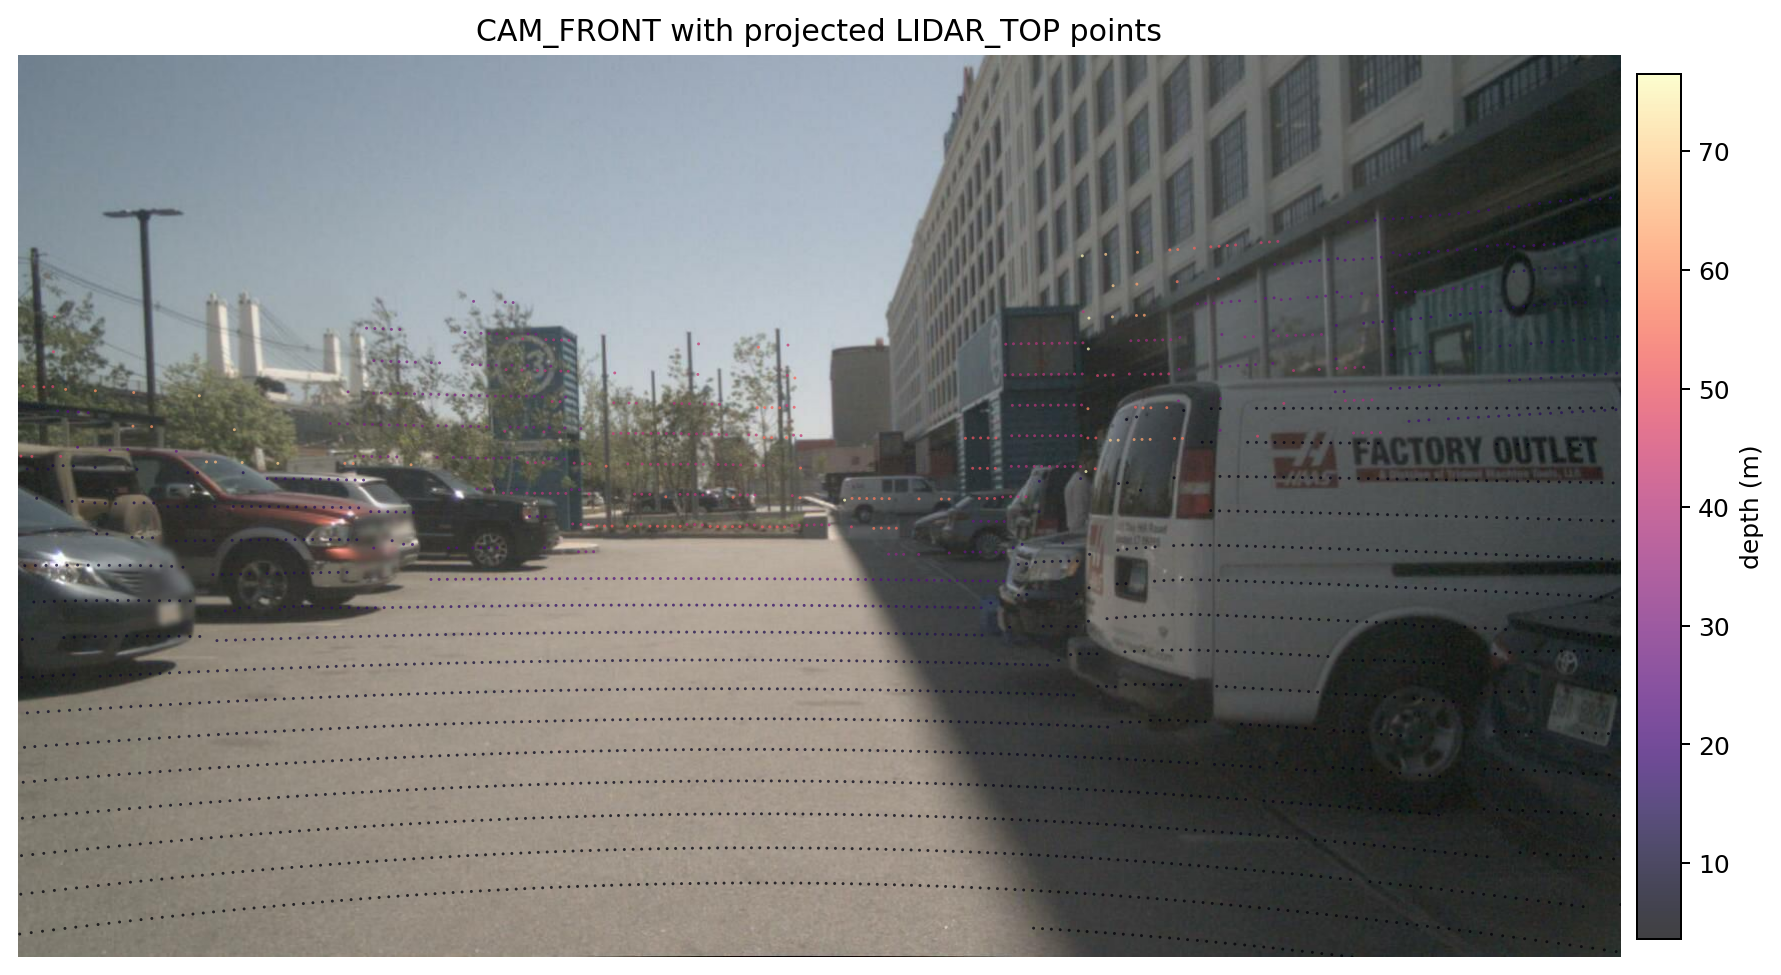
\includegraphics[width=.9\textwidth,height=7cm,keepaspectratio]{assets/overlay.png}\caption{第一次实验：LiDAR 点云投影到前视相机图像，颜色用于表示深度。}\end{figure}
该样本中共有 34720 个原始 LiDAR 点，2769 个投影到相机可见区域。点云叠加使图像语义与空间测距产生联系：道路和车辆表面的点可帮助理解深度，但稀疏区域不意味着一定没有障碍物。图中对齐质量还依赖传感器外参、位姿以及时间同步。
\begin{figure}[H]\centering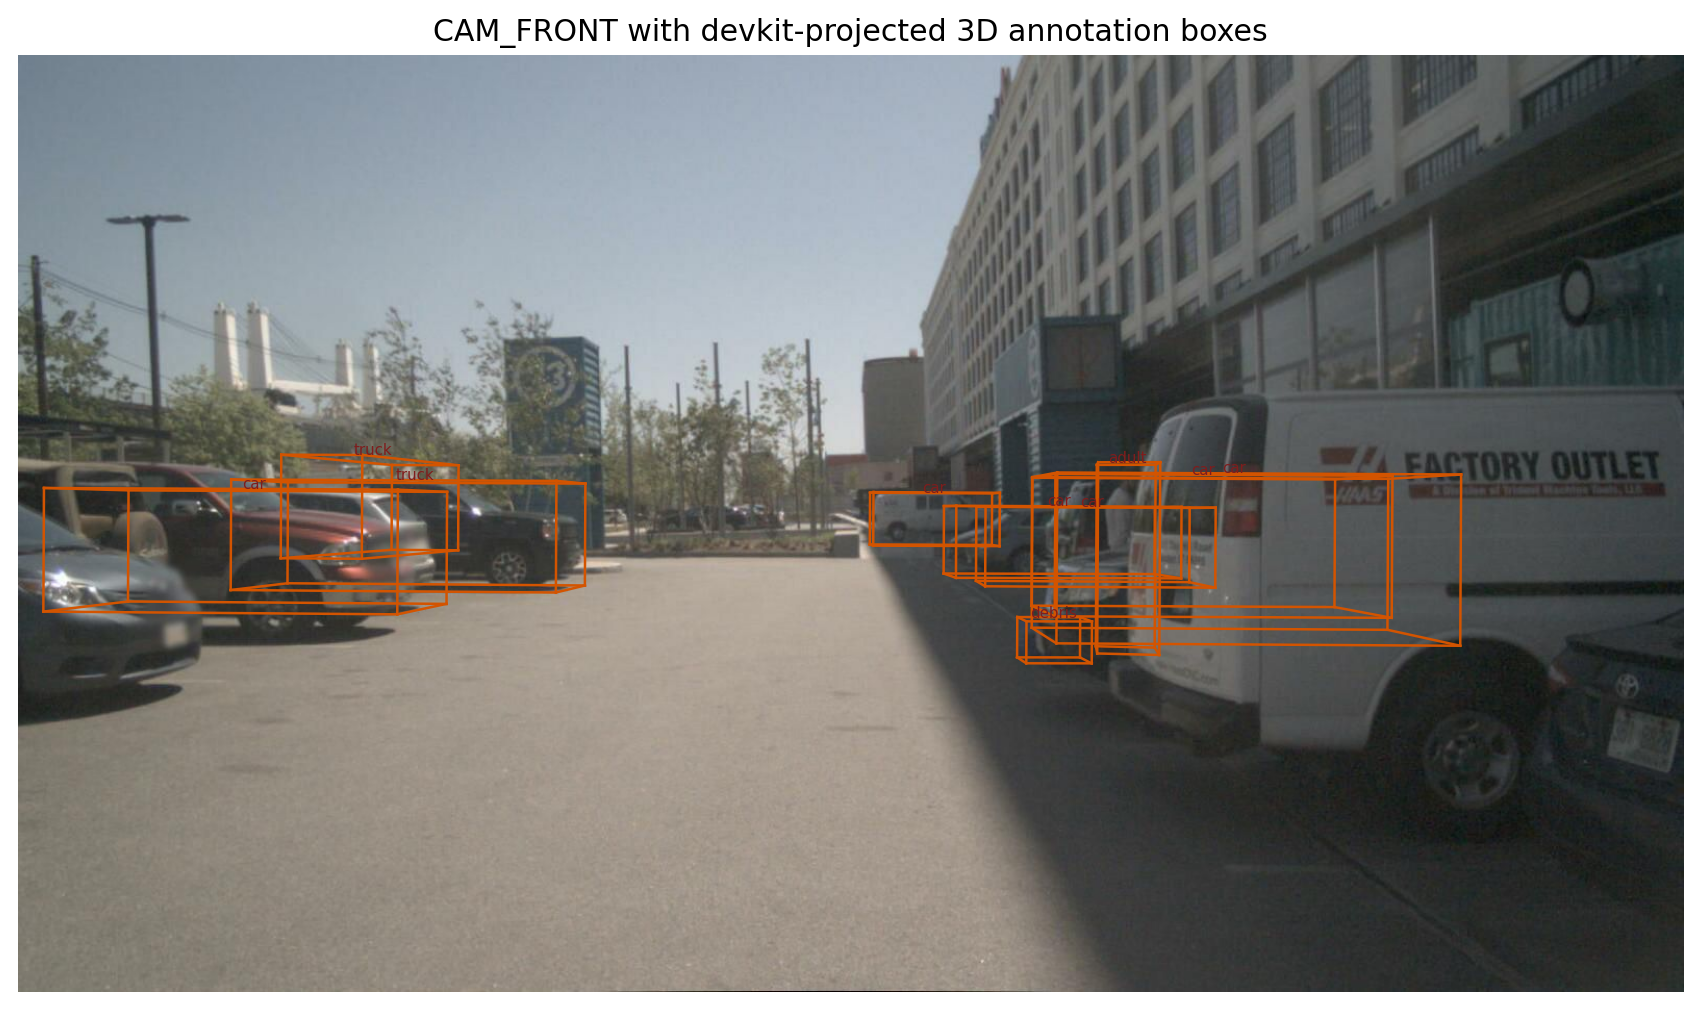
\includegraphics[width=.9\textwidth,height=7cm,keepaspectratio]{assets/projection.png}\caption{第一次实验：将三维标注框投影至前视图像。}\end{figure}
图像中的三维线框可以用于核对投影关系；训练 YOLO（You Only Look Once）系列的二维检测器时，再将投影后的可见目标转为二维外接框并归一化。这个转换会丢失朝向、深度等信息，因此二维检测得分不能回答三维定位是否准确。
\subsubsection{研究价值及长尾覆盖的限制}
nuScenes 让我能够把图像、点云、标定和三维标注放在同一套数据组织中理解，也为三维检测提供统一评估。但是“数据中包含锥桶和行人”不等于“包含足够多的施工指挥或检查配合示范”。常规目标框主要描述对象是什么、在哪里，开放问题还需要谁在指挥、指令对谁生效及应该持续多久等标注。进一步研究应结合专门场景数据，不能把通用数据集上的平均精度当成对全部道路情形的覆盖。

\FloatBarrier
\subsection{二维与三维目标检测的区别及典型算法原理}
\subsubsection{输出空间与评价指标的区别}
二维目标检测输出图像中的类别与矩形框，常用参数为 $(u,v,w,h)$；三维检测输出物体中心、尺寸和朝向，部分任务还估计速度与属性。二维框能提供语义位置，却无法唯一确定真实距离；三维结果可以直接进入空间碰撞判断，但对标定、深度或点云质量提出更高要求。二维交并比（Intersection over Union，IoU）与三维中心距离是不同的匹配标准，两类平均精度均值（mean Average Precision，mAP）的数值不应直接比较。
\subsubsection{YOLO 与 PointPillars}
YOLO11n 从图像提取多尺度特征，预测目标类别和二维框。其轻量配置适合课程训练，但单帧二维框还需要深度、跟踪或多传感器信息才能用于可靠的三维规划。PointPillars 将点云按地面网格划分为竖直柱，对柱内点编码后散射为伪图像，再用二维卷积提取特征并回归三维框。柱化将稀疏三维输入转换为适于常规卷积处理的形式，代价是对柱内高度结构作了压缩。
\subsubsection{PETR 与 BEVFormer}
PETR（Position Embedding Transformation，位置嵌入变换）将三维位置编码融入多视角图像特征，通过目标查询预测三维框；BEVFormer 在鸟瞰视图（Bird's-Eye View，BEV）网格上设置查询，利用空间交叉注意力汇聚不同相机视角，并用时序自注意力融合历史 BEV。PETR 的位置编码和 BEVFormer 的显式鸟瞰网格提供了不同的空间组织方式。后者还强调历史信息，但时序融合需要处理自车运动、目标运动和遮挡变化，并不能自动解决新场景的语义理解。

在我的修路案例中，通用检测器可以输出锥桶、工人和车辆框，BEV 表征能帮助规划理解空间关系，但还需进一步表达“这串锥桶改变了车道连接”“该人员正在要求本车等待”。因此应把目标检测与场景理解、指令识别区分开来，再设计它们如何向驾驶决策提供约束。

\FloatBarrier
\subsection{视觉与 LiDAR 目标识别实验结果及对比分析}
\subsubsection{三次感知实验的设置与指标}
表\ref{tab:experiments}按同一组维度汇总实验设置。平均精度（Average Precision，AP）经类别等维度汇总为平均精度均值（mean Average Precision，mAP）；NDS（nuScenes Detection Score，nuScenes 检测综合得分）还结合位置、尺度、朝向等误差。三种模型的输出任务、训练先验和评价匹配条件不同，先说明这些条件，再解释结果。
\begin{table}[H]\centering\small\caption{三次感知实验的条件与结果对照}\label{tab:experiments}
\setlength{\tabcolsep}{5pt}\renewcommand{\arraystretch}{1.24}
\begin{tabularx}{\textwidth}{>{\raggedright\arraybackslash}p{2.15cm}YYY}\toprule
对比维度 & YOLO11n & PETR & PointPillars\\\midrule
输入与任务 & 前视相机图像；二维框及类别 & 六路相机图像；三维框及类别 & 单帧 LiDAR 点云；三维框及类别\\
训练数据规模 & Boston 子集：9420 张训练、1402 张验证图像 & mini：8 个训练场景，共 323 帧，每帧六相机 & mini：8 个训练场景，共 323 帧单帧点云\\
最终评估数据 & 保留测试拆分 2709 张图像 & 官方 mini 验证集：2 场景、81 帧 & 同一官方 mini 验证集：2 场景、81 帧\\
预训练与更新范围 & 公开 YOLO11n 预训练权重，随后训练检测器 & 公开 ResNet50 骨干权重；检测模块从初始化训练 & 公开 PointPillars 权重；仅微调检测头\\
轮数与教学配置 & 20 轮；输入尺度 640，批大小 8 & 20 轮；六路 $192\times512$，100 查询、3 层解码器 & 累计 5 轮；批大小 1，检测平面 x/y 各方向范围 $\pm25\,\mathrm m$\\
评价指标与匹配口径 & 图像框 IoU；mAP50 及 mAP50--95 & nuScenes 三维中心距离 mAP 及 NDS & 同 PETR 的三维评估器；对照微调前后\\
实际结果 & 精确率 0.511，召回率 0.394；mAP50 0.403，mAP50--95 0.217 & mAP 0.000569；NDS 0.028768 & mAP 0.000061$\to$0.062302；NDS 0.026860$\to$0.118891\\
方法优势 & 可利用颜色、纹理和外观；本次完成较大图像拆分的识别评估 & 结合多视角与几何编码学习三维空间表征 & 输入直接包含测距信息；本次同条件微调结果改善\\
本次局限 & 没有直接输出三维距离；跨天气和遮挡鲁棒性未单独测试 & 教学数据及模型规模受限，验证检测能力很弱 & 单帧、局部范围及仅头微调；远距离小目标能力未分组测试\\\bottomrule\end{tabularx}
\end{table}
第一次实验使用 9420 张训练、1402 张验证和 2709 张测试图像；第二、三次实验使用相同的 mini 场景划分，但网络容量、预训练及优化方式不同。第一次实验保留的测试拆分也不能直接代表跨地区、跨天气或跨场景泛化；本报告只按已保存的运行记录描述结果。
\subsubsection{YOLO 图像预测与 LiDAR 鸟瞰结果}
\begin{figure}[H]\centering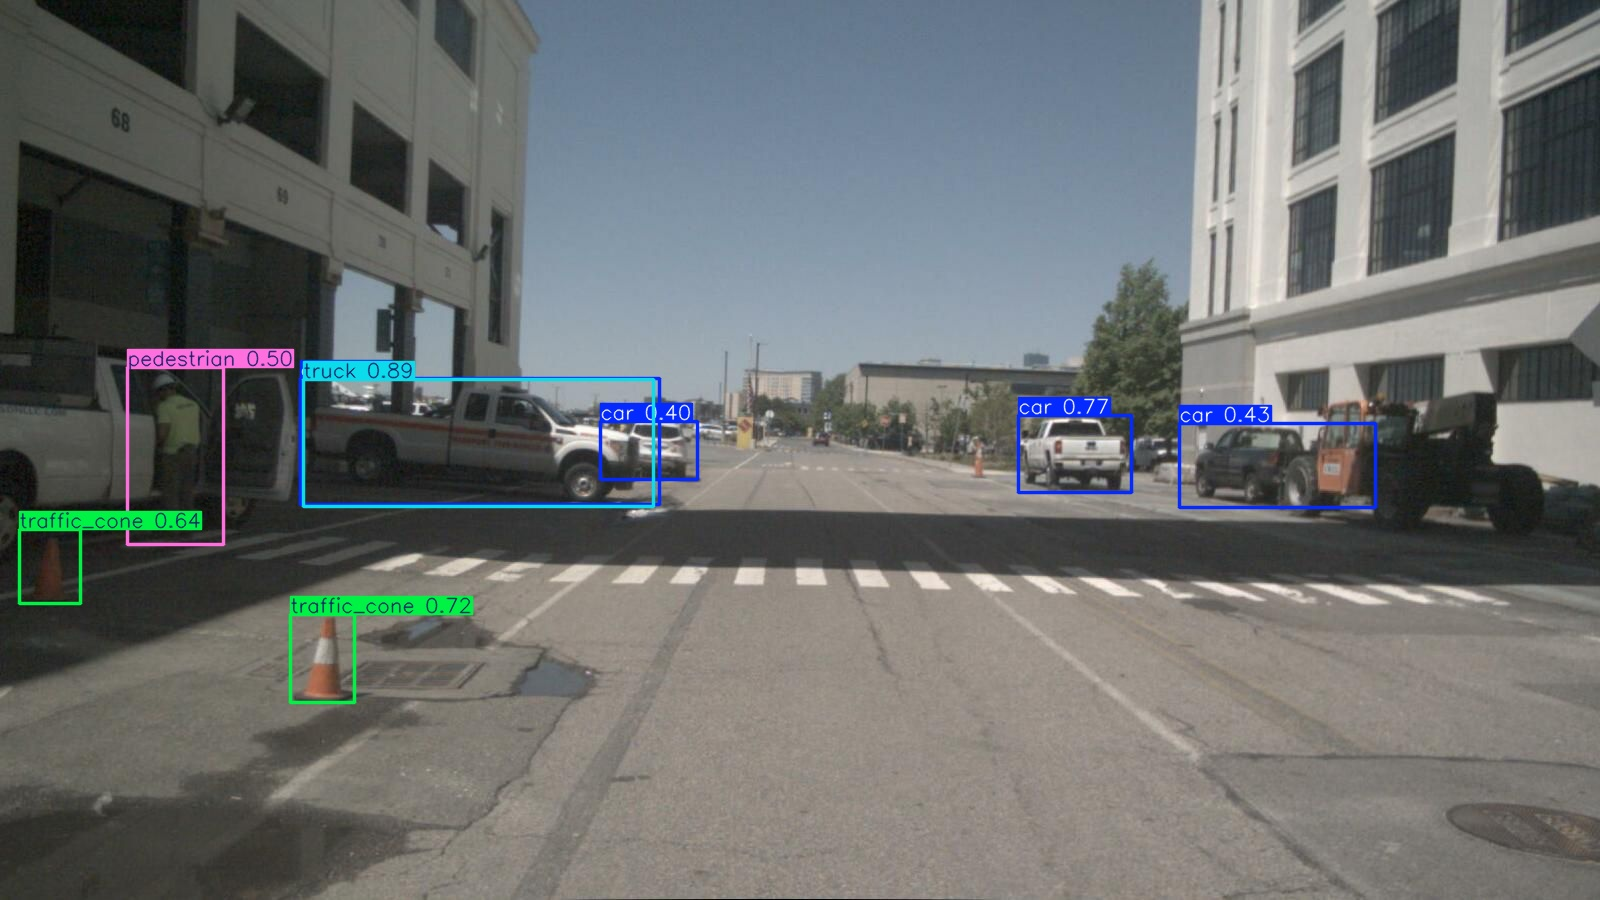
\includegraphics[width=.88\textwidth]{assets/details/yolo_example.jpg}\caption{YOLO11n 保留测试拆分中的一张原始预测图。由十二帧拼图改为单帧显示，以便辨认类别和框；选图仅用于展示。}\label{fig:yolo-result}\end{figure}
\begin{figure}[H]\centering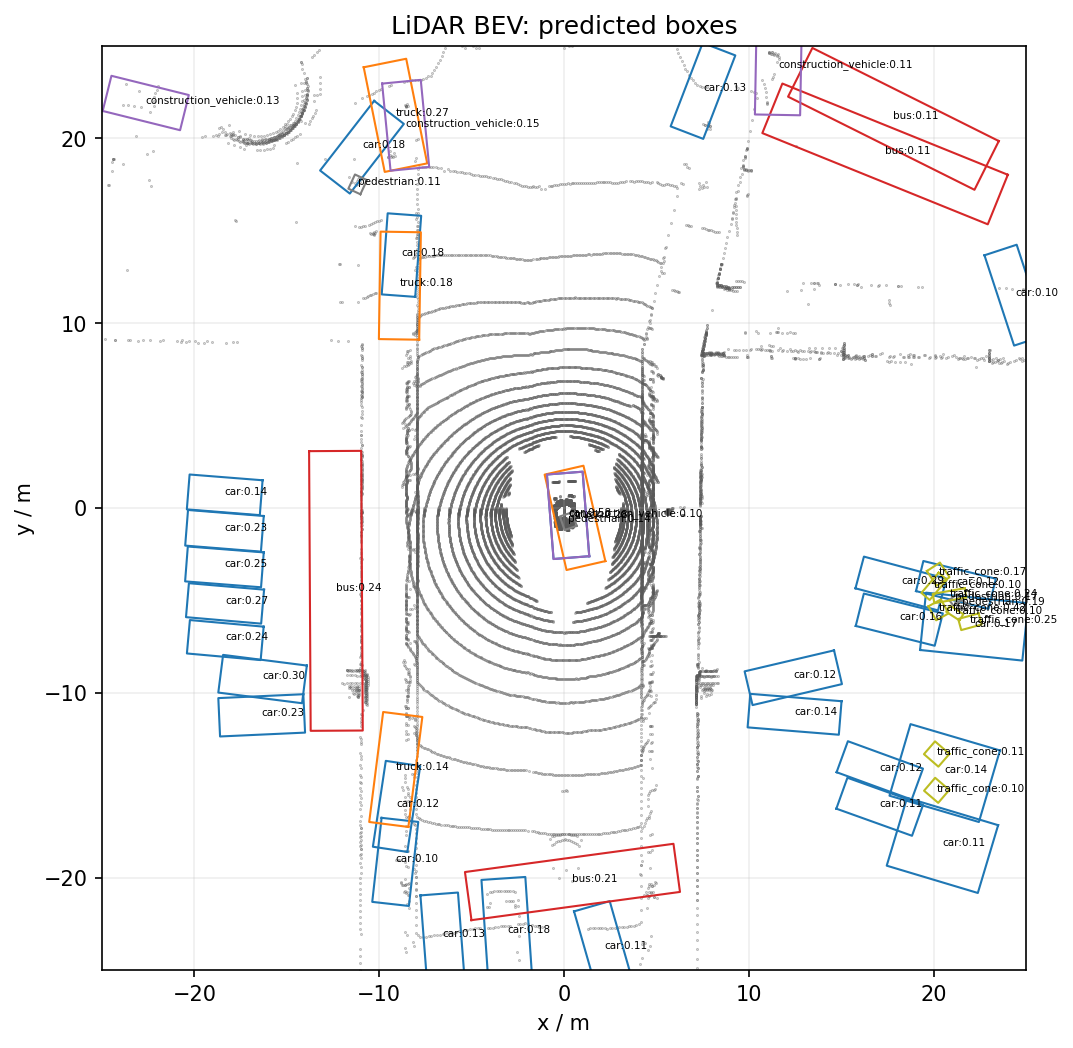
\includegraphics[width=.72\textwidth]{assets/lidar.png}\caption{PointPillars 微调后验证帧 0 的点云与预测框。横纵轴为空间位置，展示阈值为 0.10；图中未叠加真实框。}\label{fig:lidar-result}\end{figure}
图\ref{fig:yolo-result}中，YOLO 在画面里给出车辆等目标的类别和图像位置，说明视觉输入可以利用外观线索完成语义识别。但是本次召回率为 0.394，表明保留测试拆分中仍有较多标注目标未被正确检出；不能因选图中若干车辆被框出，就认为模型已经可靠覆盖小目标或遮挡目标。mAP50--95 从 mAP50 的 0.403 降至 0.217，也说明在更严格的框重叠标准下表现较弱；这与图像框定位有关，不是三维测距误差。

图\ref{fig:lidar-result}的坐标轴和点云提供了直接的空间几何参考，适合检查障碍物分布和三维框位置。微调后 mAP 为 0.062302，仍然偏低；本图又没有真实框，无法从框贴近点簇就认定检测正确。相机与点云结果来自不同场景，也没有做统一的距离、遮挡和天气分组，因此本次能确认的是各自任务的表现，尚不能量化哪种模态在同一困难条件下更好。

综合原理与这些实际结果，我认为视觉的语义优势和 LiDAR 的几何优势互补：视觉依赖颜色、纹理和外观，光照变化与遮挡可能削弱识别；LiDAR 直接提供空间点，但远距离点云稀疏，小行人、锥桶等目标可能缺少足够几何证据。这两类困难并未在本次实验中逐项验证，应作为后续分组评估的假设。融合实验可以检查视觉类别与点云位置是否互相补充，同时控制同步、标定和融合方式；若数据错位，增加传感器也可能引入错误关联。

表\ref{tab:experiments}进一步说明，YOLO 与三维检测任务使用不同指标，PETR 与 PointPillars 又有不同预训练和更新范围。只有固定场景、任务、训练资源及评价规则，才能进行模态比较；这里更有说服力的实验对照，是 PointPillars 在自身固定设置下的微调前后变化。
\subsubsection{PETR 六相机结果与失败现象}
PETR 实验先利用相机标定建立共同的三维参考，再从六路图像预测三维框。图\ref{fig:six-camera}中的图像平面位于光轴深度 8 米，仅用于显示相机间几何关系，不代表物体真实表面或场景重建。
\begin{figure}[H]\centering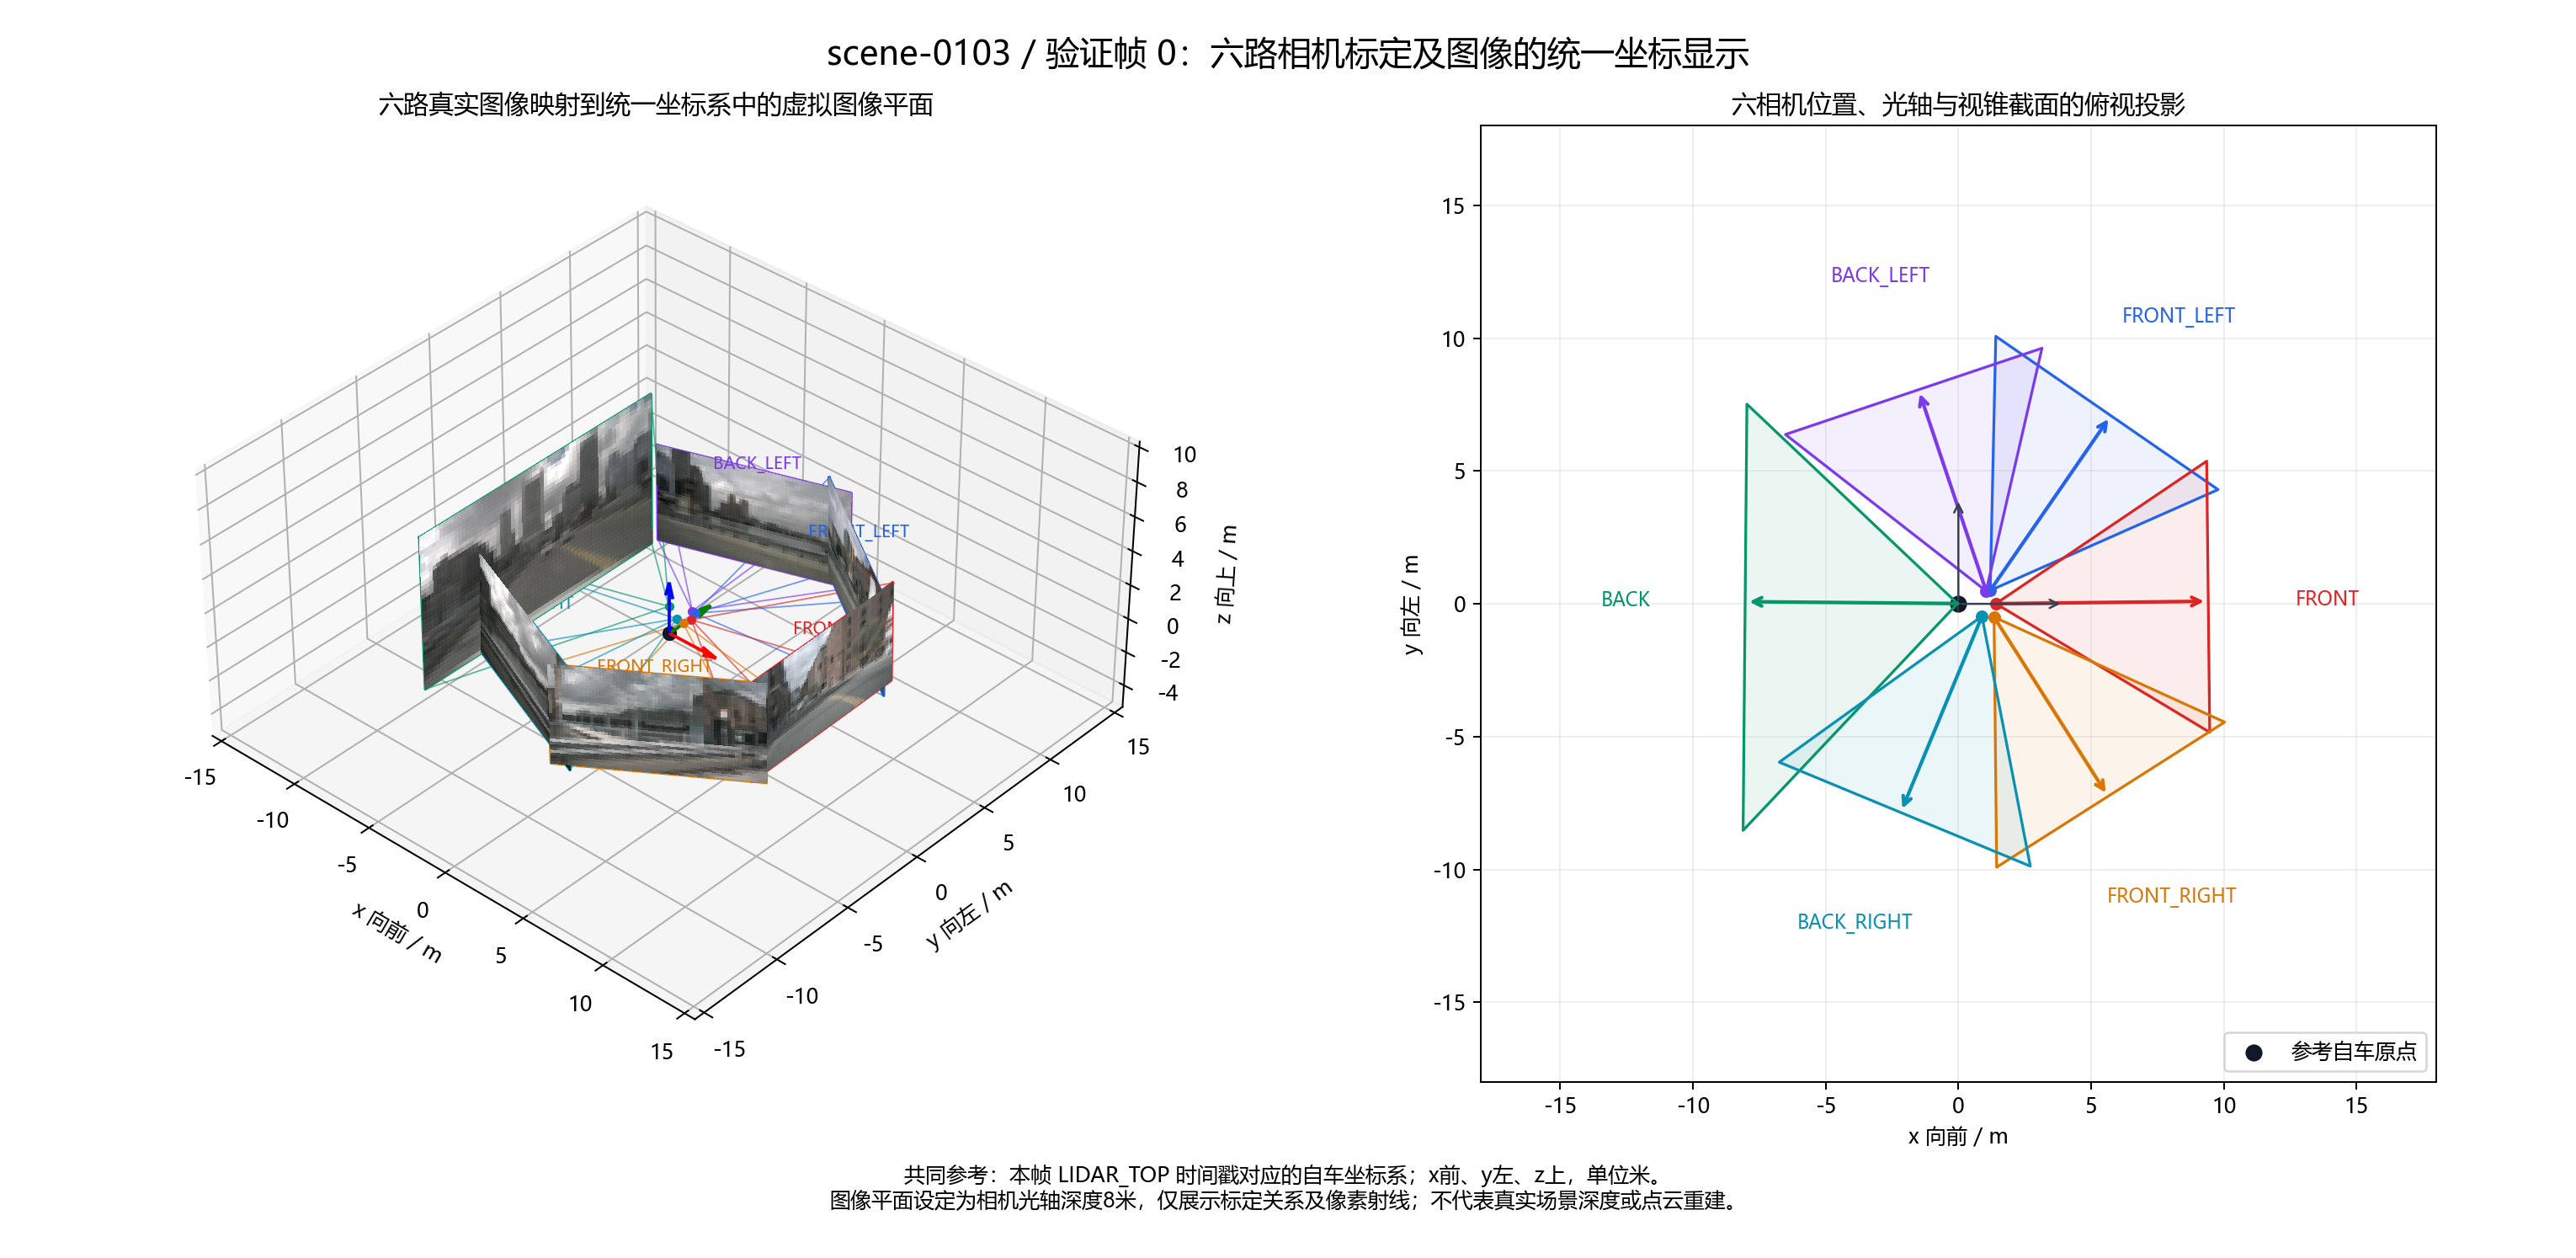
\includegraphics[width=\textwidth]{assets/six.png}\caption{六相机图像和相机位置的统一坐标显示。8 米为绘图设定的候选深度。}\label{fig:six-camera}\end{figure}
为看清错误，图\ref{fig:petr-detail}从原六相机输出中选取前视和右后视两组真实框与预测框，保留原始检测内容。前视真实框多沿车辆和行人分布，而预测框在道路等位置出现较大偏移；右后视近处行人与预测框的位置也明显不对应。框数接近并不意味着匹配正确，降低显示阈值也不能修复位置错误。
\begin{figure}[H]\centering
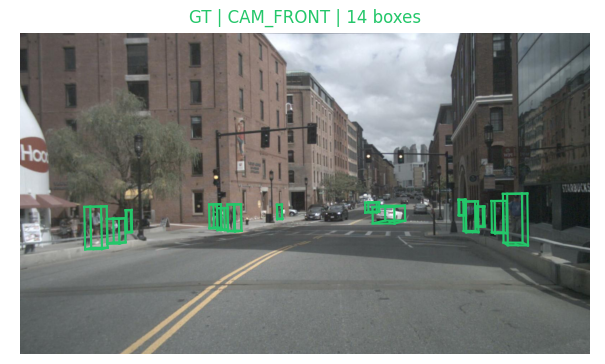
\includegraphics[width=.49\textwidth]{assets/details/petr_front_gt.png}\hfill
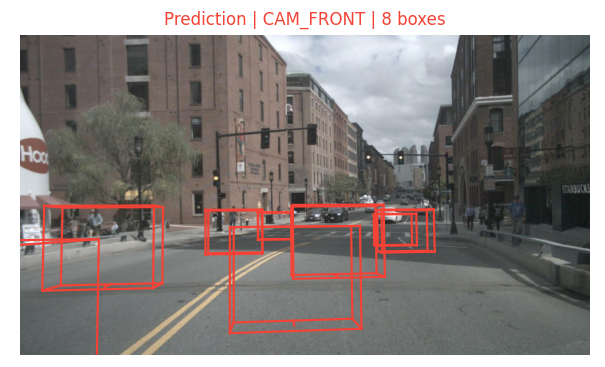
\includegraphics[width=.49\textwidth]{assets/details/petr_front_pred.png}\\[5pt]
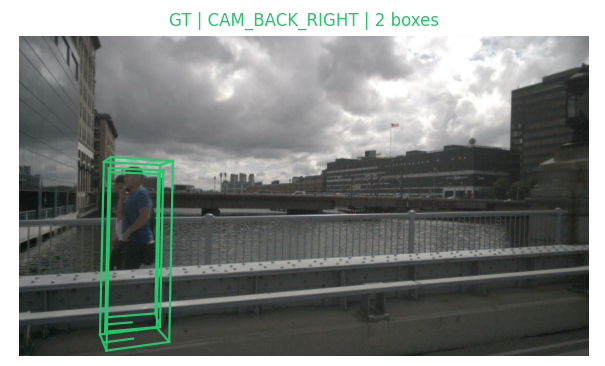
\includegraphics[width=.49\textwidth]{assets/details/petr_rear_right_gt.png}\hfill
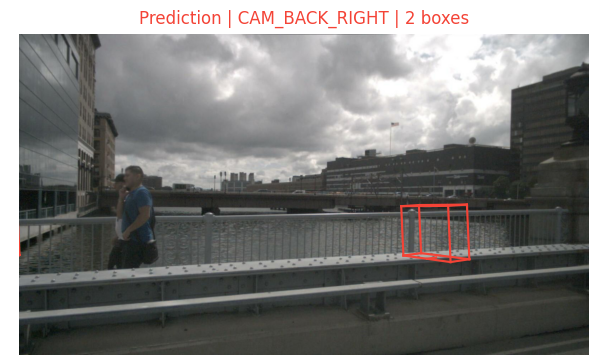
\includegraphics[width=.49\textwidth]{assets/details/petr_rear_right_pred.png}
\caption{PETR 同一验证帧的局部结果。上排为前视、下排为右后视；左列绿色真实框、右列红色预测框。由六相机结果裁切重排，未修改框；显示阈值 0.1，全帧共享前 20 个预测。}\label{fig:petr-detail}\end{figure}
81 帧格式化输出共 6783 个预测，其中 car 占 6319 个，约为 93.16\%，显示出明显的类别偏向。验证集虽缺少三个类别的有效标注，但已有行人等类别的 AP 也为零，因此类别覆盖不足不能单独解释全部低精度。图中真实框按绘图可见性筛选，数量并非评估器实际匹配数。

我把可能的影响因素分为三个层次，并将事实与解释分开。

\textbf{数据层。}已确认训练只有 323 帧，类别有效标注数不均衡，例如 car 为 4082 个、trailer 为 59 个；验证集场景也只有两个。有限覆盖和类别失衡可能使学习偏向常见类别，但尚未做采样或类别权重消融。下一步应固定模型，比较不同采样策略，并按类别和距离检查召回，而不是直接把低 AP 归因于数据少。

\textbf{模型层。}已确认教学配置使用较低图像分辨率、100 个查询和 3 层解码器，只有 ResNet50 骨干使用公开预训练，三维检测模块从初始化训练。这些设置可能限制空间细节和特征适配，但未证实哪个因素起主导作用。可先做单帧拟合检查框编码及标定链路，再分别测试分辨率、模型容量或检测预训练的影响。

\textbf{训练层。}已确认完成 20 轮、6460 次迭代，已记录批次的轮均损失由 13.408410 降至 8.723793；这证明训练目标被优化，却不能证明验证性能已经收敛。当前没有逐轮验证曲线和训练轮数消融，因而既不能断言训练轮数足够，也不能断言延长训练必然有效。后续应固定其他条件记录多轮验证、重复随机种子，并观察逐类 AP；若训练损失继续下降而验证不改善，还要检查过拟合或任务适配问题。

我的结论是，本次已经观察到类别偏向、框错位和极低验证 AP，但没有完成足以定位主因的受控实验。将三个层次分别验证，比凭经验挑选一个原因更接近可复现的实验分析。
\subsubsection{PointPillars 微调代码与自身前后对照}
PointPillars 按水平网格将点分组为柱，编码柱内点，再映射到鸟瞰平面；主干网络提取特征，检测头输出类别和三维框。第三次实验只更新检测头，以下为实际实现中设置可训练参数的关键片段，其他层保持冻结。
\par\noindent\begin{minipage}{\linewidth}
\begin{lstlisting}[language=Python,caption={PointPillars 仅训练检测头的参数选择}]
model = runner.model.module if hasattr(runner.model, 'module') else runner.model
for name, parameter in model.named_parameters():
    parameter.requires_grad = name.startswith('pts_bbox_head.')
trainable = [(name, p) for name, p in model.named_parameters()
             if p.requires_grad]
if not trainable:
    raise RuntimeError('No trainable detection head parameters')
\end{lstlisting}
\end{minipage}\par
代码中异常提示文字为便于阅读的英文改写，参数筛选逻辑与实验实现一致。参数冻结并不等于只执行检测头：冻结的骨干仍参与前向计算，只是不更新其参数。实验还在训练前后检查可训练参数变化和梯度有限性，以确认实际发生了更新。
\begin{figure}[H]\centering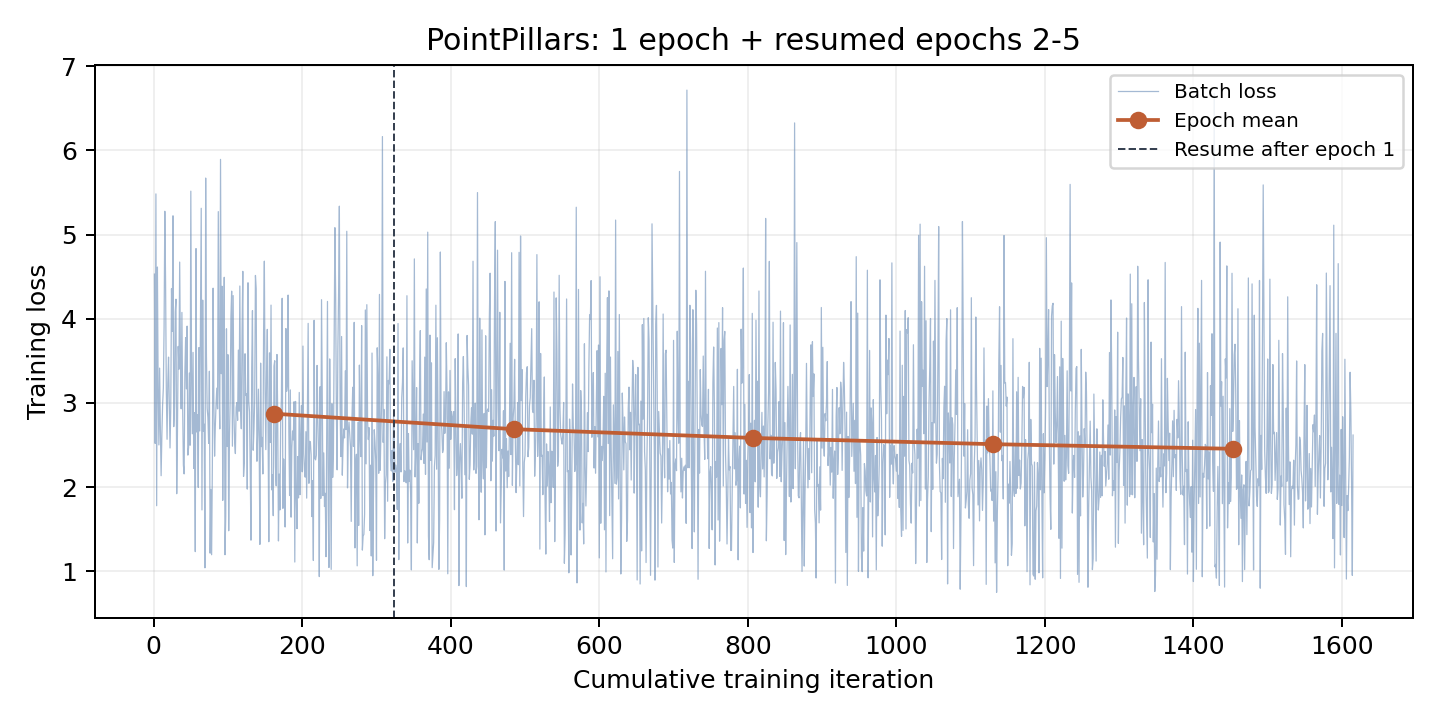
\includegraphics[width=.83\textwidth,height=6.5cm,keepaspectratio]{assets/pillar_loss.png}\caption{第三次实验：累计五轮 PointPillars 训练损失。}\end{figure}
五轮整轮平均损失从 2.873274 下降到 2.456259；同一 mini 验证集上，微调前后 mAP 从 0.000061 变为 0.062302。前者说明训练目标在优化，后者才提供了同一验证条件下的泛化证据。两次评估使用同一个小验证集，仍应警惕场景少带来的波动，且该结果不能替代完整数据集评估。
我更愿意将这组实践概括为不同任务的学习记录：YOLO 展示二维识别链路，PETR 暴露小规模配置下的三维学习困难，PointPillars 展示可核验的微调变化。要检验视觉与 LiDAR 对修路的差异，应在相同施工片段上分别报告远处锥桶召回、工人漏检、临时通道边界误差和推理延迟，并让同一规划器使用两种输出。这样才有可能把模态差异与训练条件分开。

\FloatBarrier
\subsection{复杂道路环境感知的主要问题及改进思路}
\subsubsection{施工区域需要理解临时道路结构}
复杂环境问题包括远距离小目标、遮挡、夜间眩光、雨雾、标定误差和未知类别。施工还改变了道路拓扑：原本相连的车道可能被截断，工人和设备会移动，可通行的几何空隙未必是行驶路线。单独提高锥桶检测召回率只能解决其中一部分。

我的改进重点是把分散的锥桶、工人和指示牌组织为临时通道，判断哪条车道被截断、标牌对哪里生效，以及现场信息是否与旧地图冲突。ROADWork 在国际计算机视觉大会（International Conference on Computer Vision，ICCV）2025 年论文中研究施工区识别与通行路径，正好提供了这类问题的参考，图\ref{fig:roadwork}展示了路径差异\cite{roadwork}。它支持施工语义值得专门研究，但没有证明同样的方法已适用于我遇到的道路；要迁移这一思路，仍应验证本地标牌、施工布置和工人行为。
\paperfig{roadwork}{.68}{8.1}{施工区的安全路径与不安全路径示例}{roadwork}{fig:roadwork}
\subsubsection{检查点需要理解人员指令及其适用对象}
我的酒驾检查观察提示，感知至少要区分普通行人动作、工作人员引导和要求停车的交通指令。还要判断指令是否面向本车、是否被遮挡、与上一时刻是否一致，以及是否存在明确的放行信息。夜间反光衣、强光和手臂过渡动作都会增加难度。

我认为需要同时回答两个问题：动作是什么，以及动作是否针对本车。RSC-GestureNet 对中国交警手势的研究提示，可利用过去帧和姿态可靠性判断命令，不可靠时暂不强制分类\cite{gesture}。但手势识别本身没有回答第二个问题，更没有完成检查配合。对我的案例，我会把“指令对象关联是否正确”和“停车动作是否执行”单独列为评价项，而不只看手势分类准确率。
\paperfig{gesture}{.96}{6.2}{交警手势的可靠性建模、时序识别与选择性命令输出}{gesture}{fig:gesture}
\subsubsection{从固定类别检测扩展到时空占用与未知风险}
开放道路还会出现掉落货物、变形护栏、伸入车道的异形物等，未必都属于训练时定义的十类目标。这使我进一步思考：即使模型说不准它是什么，也应尽可能判断它占据哪里、是否挡住通路，以及哪些空间还没有被可靠观测。类别置信度低与空间安全可通行不是同一个结论。

三维占用表征把空间划分为单元，描述占据情况；再加入时间，就能讨论空间随运动的变化。在三维占用空间中预测场景演化和自车运动，可以同时考虑障碍物与周围可通行空间。我认为这种表征可补充几何结构，但占用本身不能解释检查指令或路权，也不能保证被遮挡空间没有目标。

如果继续感知实验，我会把“已观测为空、已占据、观测不足”分开处理，并设置不在训练类别内的障碍来检验。评价除类别精度外，还应包括障碍边界、可用通行宽度、未知空间误判为空的次数和最终通行风险。开放词汇模型可提供语义线索，但不能只因为它能给物体取名，就认为已经完成可靠的距离和风险估计。

\subsubsection{把改进思路变成可验证的实验}
我会先建立按场景组织的错误清单，再分阶段增加能力：第一阶段补齐工人、施工设施和文字等感知信息；第二阶段建立车道封闭、停车引导及放行等关系；第三阶段把低可信度结果传给规划器。降低置信度阈值能增加显示框，未必能减少危险误判，因此不能把“画得更多”当作改进。
\begin{table}[H]\centering\small\caption{拟议感知改进实验及其评价重点，均为后续方案}
\begin{tabularx}{\textwidth}{p{2.3cm}XX}\toprule
改进项 & 对照方式 & 应观察的结果\\\midrule
时序与跨模态融合 & 单帧与多帧；相机与相机加 LiDAR & 遮挡恢复、位置误差、延迟及模态缺失退化\\
施工场景语义 & 仅检测框与增加通道及标牌关系 & 封闭区误通行、通道边界错误、地图冲突识别\\
人员指令理解 & 单帧动作与连续命令及对象关联 & 停止误识为通行的次数、指令延迟、拒识情况\\
不确定性输出 & 固定置信度与可靠性校准 & 置信度与实际错误是否一致，规划是否合理降级\\\bottomrule\end{tabularx}\end{table}
进一步可以扩展到事故现场、救援人员挥手、校门口引导和雨夜遮挡。它们与修路、检查点共享一些感知能力，但需要分别检验。尤其应关注高风险混淆：把“停车”等待误解为“可以绕行”，通常比把不确定指令暂时保留更值得优先分析。

\section{自动驾驶规划决策与端到端自动驾驶综合分析}
\FloatBarrier
\subsection{如何实现自身定位路径规划和驾驶决策}
\subsubsection{融合定位与地图匹配}
定位估计自车的位置、姿态和运动状态。GNSS 提供绝对参考，IMU 和轮速计补充短时运动，视觉或 LiDAR 里程计利用环境特征估计相对位移，再通过地图匹配和滤波或优化降低漂移。城市峡谷、隧道和重复纹理可能使定位退化，系统应把位姿不确定性传给规划器，而不是继续把地图匹配结果当作精确事实。

修路时应区分“自己在地图哪里”和“地图上这条路现在还能否通行”。即使定位准确，旧地图也可能没有临时围挡；反过来，看到围挡也不意味着全球定位失效。我的改进思路是保留全局导航方向，同时依据现场信息更新局部车道连接和通行约束，必要时重新规划路线。
\subsubsection{全局路径局部轨迹与行为决策}
全局路径规划在路网中搜索通向目的地的道路序列，可使用 Dijkstra 或 A* 等方法。局部轨迹规划根据实时环境求解未来数秒的车辆位置、速度和加速度序列，约束包括道路边界、障碍物、车辆动力学和可用制动能力。行为决策位于任务和轨迹之间：同一个目的地可以对应跟车等待、借道绕行或先停车等不同行为。

一种便于理解的规划表述为：
\begin{equation}
\min_{\tau\in\mathcal F}\ \lambda_p J_{\mathrm{progress}}(\tau)+\lambda_c J_{\mathrm{comfort}}(\tau)+\lambda_i J_{\mathrm{interaction}}(\tau),
\end{equation}
其中 $\tau$ 为候选轨迹，$\mathcal F$ 表示满足碰撞、道路及当前场景约束的可行集合。这个式子是本文的说明性概括。风险约束不宜完全靠增加一个软惩罚权重实现，否则模型仍可能用更高通行效率抵消危险代价；具体约束如何保证有效，仍取决于感知误差和车辆模型。
\subsubsection{从避障扩展到有状态的交互决策}
酒驾检查场景可抽象为“接近并确认引导、减速停车、持续等待、确认放行、恢复行驶”的状态序列。若只优化目的地进度，检查人员和锥桶可能被当作需要绕过的对象；把停车等待作为独立任务，才能解释为什么车辆应在前方有空间时仍保持停止。系统还需处理指令是否针对本车、动作不清楚及放行后路径被行人占用等情况。

下面给出说明性决策伪代码，用于表达任务状态与轨迹约束的关系；它不是实验四已有实现，也没有进行车辆验证。
\par\noindent\begin{minipage}{\linewidth}
\begin{lstlisting}[language=Python,caption={临时管制中的任务状态与轨迹约束示意}]
if scene.requires_stop and scene.applies_to_ego:
    state = "APPROACH_STOP"
if state == "APPROACH_STOP" and vehicle.is_stopped:
    state = "WAIT"
if state == "WAIT":
    if scene.release_confirmed and scene.path_is_safe:
        state = "RESUME"
    else:
        constraints.hold_position = True
if scene.command_is_ambiguous:
    request_human_review()
trajectory = plan(state, scene, constraints)
\end{lstlisting}
\end{minipage}\par
这段示意隐藏了最难的部分：如何可靠地得到 applies\_to\_ego 和 release\_confirmed。如果只是把不可靠的分类标签换成几个状态，系统依然会失败。因此应同时验证语义证据、状态转移和执行动作，并为人类接管留出实际时间。

\FloatBarrier
\subsection{端到端自动驾驶定义及与传统模块化的区别}
\subsubsection{系统架构与工作原理对比}
端到端自动驾驶将传感器、导航和自车状态映射为轨迹或控制量，围绕驾驶目标联合学习，可保留中间表征及辅助任务。传统模块化显式划分感知、预测、决策、规划和控制接口，通常可分别开发与测试。
\begin{table}[H]\centering\small\caption{两种架构在开发验证安全性与可解释性方面的比较}
\begin{tabularx}{\textwidth}{p{2.0cm}XX}\toprule
比较维度 & 传统模块化 & 端到端学习\\\midrule
中间表征 & 框、地图、预测等接口明确，便于逐级检查 & 依赖学习表征，也可保留中间任务\\
优化目标 & 分别优化模块，再进行系统调试 & 驾驶目标与辅助监督联合优化\\
故障定位 & 较易追踪到模块和接口，仍需检查耦合 & 可跨任务协调，内部决策归因较难\\
安全约束 & 可在接口和规划层显式施加约束 & 结合训练、轨迹约束与独立安全监测\\
解释的可检验性 & 可追溯过程，仍须验证最终动作 & 表征较难解释，语言说明须与轨迹核对\\
数据依赖 & 各模块可分别训练调试，仍依赖数据覆盖 & 通常依赖更大数据及训练体系，可分阶段训练\\
新场景适配 & 可补规则或模块，维护复杂度增加 & 靠数据学习，受覆盖与泛化限制\\
验证需求 & 模块与闭环测试，检查误差传播 & 闭环行为验证，检查风险与动作一致性\\\bottomrule\end{tabularx}\end{table}
\begin{figure}[H]\centering
\begin{tikzpicture}[b/.style={draw,rounded corners,align=center,minimum height=11mm,font=\small},a/.style={-{Stealth},thick}]
\node[anchor=east,font=\small\bfseries] at (-.6,0) {模块化};
\node[b,text width=22mm](a) at (.8,0){传感器};
\node[b,text width=25mm](b) at (3.6,0){感知与定位};
\node[b,text width=25mm](c) at (6.6,0){预测与规划};
\node[b,text width=25mm](d) at (9.6,0){控制与执行};
\draw[a](a)--(b);\draw[a](b)--(c);\draw[a](c)--(d);
\node[anchor=east,font=\small\bfseries] at (-.6,-1.9) {端到端};
\node[b,text width=22mm](e) at (.8,-1.9){传感器\\导航与状态};
\node[b,text width=54mm](f) at (5,-1.9){联合训练的驾驶模型\\可包含中间表征及任务监督};
\node[b,text width=25mm](g) at (9.6,-1.9){轨迹或控制\\车辆执行};
\draw[a](e)--(f);\draw[a](f)--(g);
\end{tikzpicture}\caption{传统模块化与端到端自动驾驶架构对比。两者均需要执行反馈和系统监测。}\label{fig:compare}\end{figure}
表中的可解释性与安全性需要分开看：能定位到某个模块，有助于排错，但不自动保证闭环安全；能给出流畅的驾驶解释，也不证明轨迹确实服从解释中的风险判断。两种架构都需要检查输入可靠性、规划约束和执行反馈；显式约束的有效性也依赖状态估计，不能单凭约束写在程序里就认为已经安全。
\subsubsection{课程行为克隆实验与关键代码}
第四次实验是行为克隆的简化例子：网络由前视图像回归转向，服务端另根据当前速度和转向计算油门，并非完整的城市端到端驾驶系统。训练 30 轮后，6489 张验证图像上的 均方误差（Mean Squared Error，MSE） 为 0.077897、平均绝对误差（Mean Absolute Error，MAE）为 0.207337。验证集参与选模，且按记录随机划分，相邻帧可能相似；合成客户端仅证明一次服务请求可返回控制值，模拟器窗口未能激活，因此没有闭环碰撞率、偏离率或安全行驶结论。
\begin{figure}[H]\centering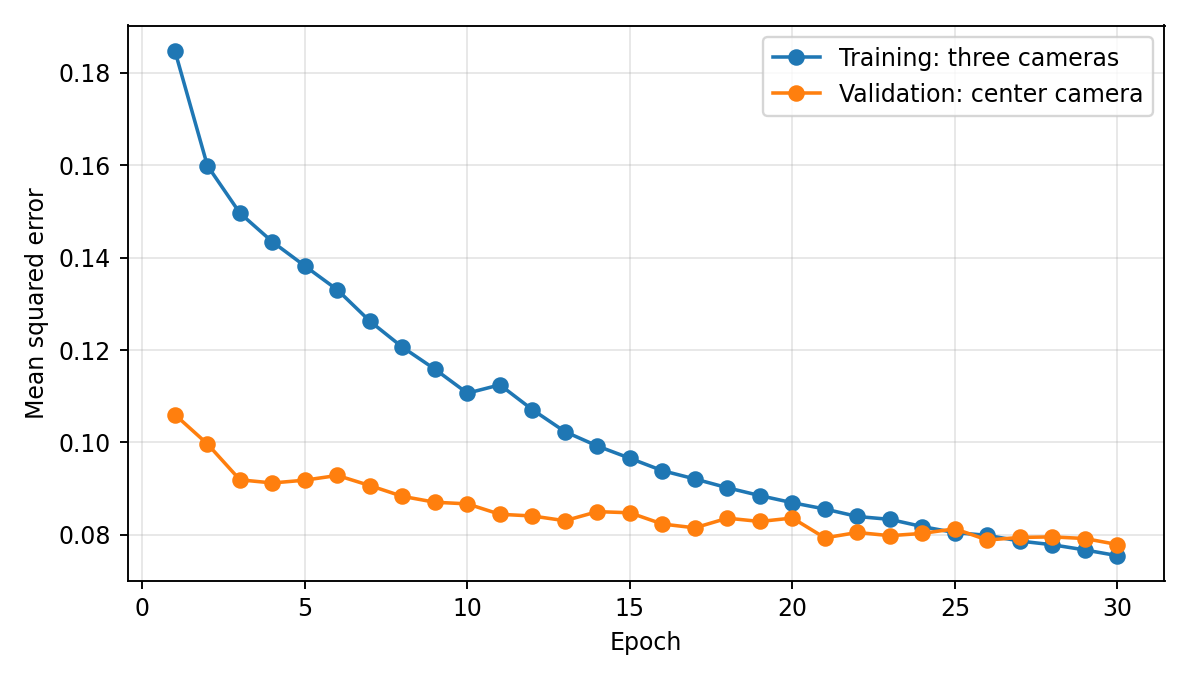
\includegraphics[width=.78\textwidth,height=6cm,keepaspectratio]{assets/driving.png}\caption{第四次实验：30 轮行为克隆训练与验证损失。}\end{figure}
实验四以驾驶记录中的图像和转向角为监督。训练数据按记录随机划分，训练使用左、中、右相机并施加转向修正，验证仅使用中央相机；水平翻转时同时反转转向标签。下面摘录训练数据读取中的关键步骤，变量与原实现一致，省略了路径读取及异常处理。
\par\noindent\begin{minipage}{\linewidth}
\begin{lstlisting}[language=Python,caption={行为克隆的数据增强和输入归一化}]
angle = float(row[3]) + (0, .4, -.4)[camera]
img = img[65:-25]
if self.train and random.random() < .5:
    img = cv2.flip(img, 1)
    angle = -angle
img = np.ascontiguousarray(
    (img.astype(np.float32) / 127.5 - 1).transpose(2, 0, 1))
return torch.from_numpy(img), torch.tensor([angle], dtype=torch.float32)
\end{lstlisting}
\end{minipage}\par
左右相机的 $\pm0.4$ 是课程实现中用于模拟偏离车道后的转向修正，并非从真实轨迹反算出的普适标定值；裁剪、颜色通道顺序和归一化必须在训练和服务推理时保持一致。训练使用均方误差优化预测转角与记录转角的差异，但驾驶记录常包含大量接近直行的帧，模型可能更擅长常见工况而忽视急弯和纠偏。
图\ref{fig:steering-pred}中颜色体现样本密度而非单个轨迹的时间顺序。接近虚线说明部分样本误差较小，偏离虚线的区域提示特定转角可能预测不足或偏差较大；由于验证集参与选择最优权重且相邻帧相关，这幅图不能代表未见道路上的闭环表现。下一步应以完整赛道或驾驶片段划分独立测试集，启动模拟器后统计车道偏离、碰撞和恢复能力，并记录失败场景及复现条件。

对检查点而言，图像到转向的单一回归目标尤其不足：停车需要纵向控制，等待需要记忆状态，放行需要理解时序交互。这也解释了为什么实验四可以帮助理解端到端映射，却不能从转向误差推断它已经具备城市道路综合驾驶能力。
\begin{figure}[H]\centering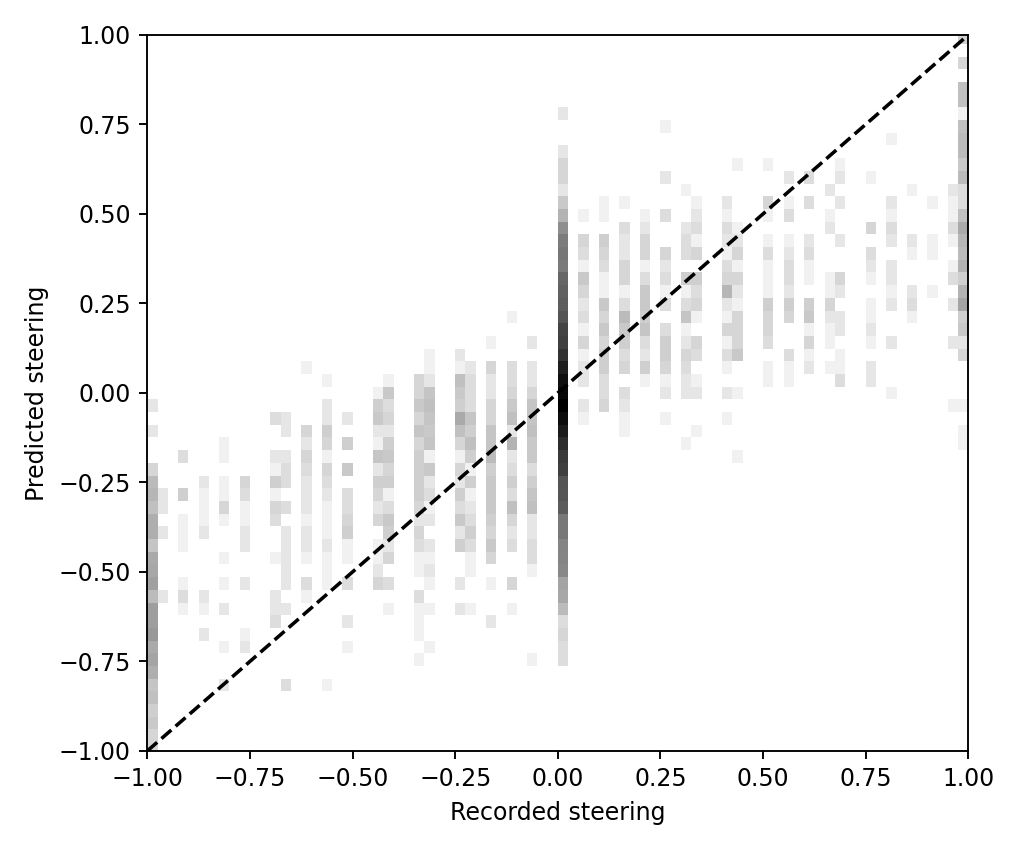
\includegraphics[width=.76\textwidth,height=7cm,keepaspectratio]{assets/predictions.png}\caption{第四次实验：验证集记录转角与预测转角的二维频次图，虚线表示预测值等于记录值。}\label{fig:steering-pred}\end{figure}

\subsubsection{前沿模型中的推理与动作连接}
对检查点这类任务，我最关心的是“停车理由是否真正进入动作”，因此不能只评估解释是否合理。Alpamayo-R1 将推理与轨迹生成连接，并训练两者的一致性，图\ref{fig:alpamayo}给出了一条技术路径\cite{alpamayo}。它对我的启发是给模型增加决策理由与动作关联的训练和测试，而不是依靠网络规模来推断理解能力；论文自身的测试也不能直接证明其覆盖了我的检查配合场景。
\paperfig{alpamayo}{.90}{5.0}{视觉编码、推理骨干与轨迹生成的连接}{alpamayo}{fig:alpamayo}
一种后续测试是保留相似道路和车辆状态，只改变“普通行人”与“明确要求本车停车的指挥者”这一条件，观察纵向轨迹、停车点和等待行为是否相应变化。该测试是本文提出的方案，不能仅根据模型生成的解释判断它已经理解了交通场景。

综合架构和实验，我更倾向于按任务组合方法：用学习模型提取场景信息或生成候选轨迹，用可检查的约束筛查风险，再由控制器闭环执行。端到端可以保留中间模块，传统模块化也仍有接口清晰和便于局部验证的价值；混合架构的意义在于发挥各自作用，并验证它们共同形成的行为。

\FloatBarrier
\subsection{城市道路前方行人突然横穿的两类系统处理方式}
\subsubsection{模块化系统的感知定位决策与控制链路}
设想车辆在城市道路行驶，行人从停放车辆后进入车道。感知系统检测并跟踪行人，定位与自车状态估计提供速度和运动方向；系统将行人位置转换到与规划一致的坐标系，并保留横穿、停顿或返回等可能轨迹。决策层根据冲突风险选择让行或紧急停车，规划层计算减速轨迹，控制层执行制动并监测减速度是否达到预期。

这一过程还需检查侧后方车辆及道路边界。突然转向可能把前向风险转移到旁边的骑行者，不能把“避开这个行人”作为唯一目标。若有充分视距，系统应尽早平顺减速；若已经进入紧急状态，则以实际可行的风险降低动作处理，并持续更新预测。控制反馈用于修正制动效果，不能假设发出制动指令就已经停止。
\subsubsection{端到端系统及感知动作一致性问题}
端到端模型可依据连续图像、自车状态和导航指令输出减速轨迹或控制动作，也可利用中间占用、预测或风险表征。它同样受到可见距离、计算延迟与车辆制动能力约束。训练中出现过类似横穿样本，有助于学习反应，但并不能保证在不同遮挡和车速下都正确响应。

\begin{table}[H]\centering\small\caption{行人横穿场景的阶段决策对照，端到端内部形式随具体架构而异}\label{tab:crossing}
\begin{tabularx}{\textwidth}{p{1.8cm}XX}\toprule
阶段 & 模块化系统 & 端到端系统\\\midrule
目标出现 & 检测跟踪行人，估计位置及运动 & 从连续观测形成驾驶表征，可含检测头\\
风险判断 & 预测行人轨迹及与自车的时空冲突 & 结合观测与自车状态形成风险表征，可含辅助预测头\\
行为选择 & 选择让行或紧急制动，规划减速轨迹 & 生成减速轨迹或控制量，并检查可行约束\\
车辆执行 & 执行制动，反馈车速及执行误差 & 由控制器执行模型输出并反馈车辆状态\\
后续处理 & 持续跟踪，确认冲突解除后再恢复 & 依据新观测更新动作，持续让行或恢复\\\bottomrule\end{tabularx}\end{table}
我的判断是，两种架构的核心差别在于如何将环境信息转化为可靠的驾驶动作，以及如何验证动作确实响应了风险。识别行人是必要环节，但还应继续追问：行人更近、遮挡更强或车速更高时，计划是否相应改变，实际车辆是否及时减速。


为区分这些问题，可以先固定车速和道路，只改变行人位置，检查轨迹是否响应。Perceives but Doesn't Brake 的受控研究发现，危险信息可能存在于表征中却没有充分影响纵向动作，为这种诊断提供了参考\cite{binding}。我希望借鉴的是逐层检查证据到动作的联系；该研究针对特定模型和条件，并没有证明所有端到端系统都具有同一失效原因。
\paperfig{binding}{.96}{6.1}{感知与动作连接不足及采样阶段干预示意}{binding}{fig:binding}
对我的检查点案例，需要同时保留两种解释：一是停车指令尚未被正确理解，二是相关证据已经可用却没有足够影响动作。前者需要补充场景和指令理解，后者需要检查规划目标和风险约束；在没有内部记录的情况下，我不能替产品判定是哪一种。
\subsubsection{防御性驾驶应在行人出现之前开始}
我所说的“智驾偏自我”，可以进一步转化为可观察的问题：是否只沿自己的路线前进、是否默认他车会让行、是否在遮挡出口仍保持缺少余量的速度。防御性驾驶要求对他人的可能失误和不可见风险留有余量，例如经过停放车辆、公交车站或学校出口时，提前考虑可能突然出现的人，而不是等检测到目标后才处理。

我会将“遮挡后可能出现人”作为独立风险，而不是等待出现完整检测框再行动。遮挡感知应急规划研究对潜在车辆准备探索和备用轨迹，图\ref{fig:occlusion}说明了保留后备动作的思路\cite{occlusion}。我借鉴的是提前留余量的方法；论文主要研究遮挡车辆，不能直接套用其运动边界描述行人，迁移时还需要验证行人速度和方向变化。
\paperfig{occlusion}{.53}{7.6}{遮挡路口中的探索轨迹与备用轨迹}{occlusion}{fig:occlusion}
为说明提前减速为何重要，可用简化停止距离模型：
\begin{equation}
d_{\mathrm{stop}}=v\Delta t+\frac{v^2}{2a}+m,
\end{equation}
其中 $v$ 为车速（计算时用 $\mathrm{m/s}$），$\Delta t$ 为感知至制动响应的总延迟，$a$ 为假设可维持的减速度，$m$ 为余量。若仅作教学计算，取 $\Delta t=0.3\,\mathrm{s}$、$a=5\,\mathrm{m/s^2}$、$m=2\,\mathrm{m}$，则 30 千米每小时约需 11.4 米，50 千米每小时约需 25.5 米。参数不来自本次车辆实测，模型也未考虑坡度、附着变化及制动建立过程，不能作为实际车辆的速度设定依据。

这个算例说明，在有限视距下提前降低速度，比等待危险出现后再追求更快反应更有意义。但防御性驾驶也不等于对所有可能性永久停车：系统需要利用低速观察获得新信息，在风险下降后及时恢复通行。否则可能在无冲突时反复急停、诱发后车风险，或与其他车辆互相等待形成僵局。

\FloatBarrier
\subsection{当前发展水平存在问题及未来方向的认识}
\subsubsection{从个人观察到可以检验的能力边界}
我对当前智驾的直观感受是，基础路段的行驶已经很稳定，但面对修路、酒驾检查等临时情境，处理仍不够自然；有时能够避开物体，却不能完成场景真正要求的任务。同时，系统的驾驶方式偏重本车行进，缺少我期待的防御性预判。这是我的使用观察，没有统一里程、软件版本和场景抽样记录，不能当作全部产品的统计结论。

这些现象让我更关注任务理解和交互能力。基础车道保持主要需要在已知道路结构中持续控制，临时场景则可能改变通行规则、行动目标和恢复条件。检验“能否开过去”之外，还应观察“是否应当先停、是否让别人有可预期的反应空间”。基础路段的平顺程度与罕见事件的处理水平，应分开描述。
\subsubsection{进一步延伸的长尾场景与共同问题}
\begin{table}[H]\centering\small\caption{由使用观察延伸的分析场景及能力要求，后四行为假设案例}
\begin{tabularx}{\textwidth}{p{2.1cm}XX}\toprule
情境 & 容易出现的局限 & 需要检验的能力\\\midrule
临时施工 & 沿旧车道线前进，或只绕开单个锥桶 & 更新临时通道，识别工人和指示关系\\
检查配合 & 看到人员和障碍但未形成停车任务 & 理解对象指向、停车等待和放行条件\\
救援车辆及事故现场 & 只维持原路线，不理解临时让行 & 场景识别、提前留空及受控等待\\
公交车或停放车遮挡 & 只按当前可见目标判断安全 & 潜在风险预测、视距约束和备用动作\\
狭窄道路会车 & 双方都只推进，或同时停住不再更新 & 互相影响的预测、可预期让行和僵局恢复\\
雨夜临时标线 & 对模糊指示过度确信，或反复急停 & 不确定性识别、平顺降级及接管沟通\\\bottomrule\end{tabularx}\end{table}
这些情境可以归纳为四个研究问题：现场变化能否覆盖旧先验，人员意图能否转化为本车任务，不可见风险能否影响当前速度，以及车辆能否让其他参与者理解自己的动作。这里的“沟通”不一定依赖外部显示屏，也可以体现为适时减速、保持稳定让行和不突然抢行等可预测行为。

同时需要警惕“安全”目标的片面化。过于激进会把风险留给其他人，过于保守也会造成突兀制动和通行僵局。我的判断是，防御性驾驶应追求对不确定性的适当响应：证据不足时保留余量，证据变化后及时调整，并评价对周围交通的影响。
\subsubsection{视觉语言动作与世界模型如何支持前瞻规划}
除修路和检查点外，近期值得关注的研究问题是：车辆能否在行动前比较不同选择的后果。视觉语言动作模型（Vision-Language-Action Model，VLA）把视觉、语义与驾驶动作连接起来；世界模型则尝试预测环境如何演化。两者结合的价值应体现在“不同动作会带来什么变化”，而不只是生成一段合理的语言或逼真的视频。

DriveWorld-VLA（2026）研究在潜在状态空间中连接未来场景建模与驾驶规划，使候选动作能够影响对未来的预测\cite{driveworld}。这一方向启发我把课程中的“当前帧检测”进一步扩展为“动作条件下的未来状态”。可以用下式说明这种关系：
\begin{equation}
\hat{s}_{t+k}=F_\theta\!\left(s_t,u_{t:t+k-1}\right),
\end{equation}
其中 $s_t$ 是当前环境与自车的状态表征，$u_{t:t+k-1}$ 是候选动作序列，$\hat{s}_{t+k}$ 是模型预测的未来表征，$F_\theta$ 是学习到的预测函数，$k$ 为预测步数。预测结果仍有误差，不能当作将必然发生的未来。
图\ref{fig:world-planning}展示了论文如何把共享表征、动作条件和反馈联系起来。三个阶段的区分使我能更清楚地检查：模型学到未来表征后，是否又学到了动作对未来的影响，以及这种影响是否真正参与规划。
\paperfig{driveworld}{1.0}{8.8}{世界模型与驾驶规划的联合训练、动作可控性微调及反馈完善}{driveworld}{fig:world-planning}
我认为关键检验是保持同一初始场景，改变减速、等待或变道动作，看预测的相对运动是否合理变化。如果不论怎样操作，模型都生成相似的安全画面，它就没有为决策提供有效依据。将世界模型用于闭环训练前，需要验证模拟结果是否随动作变化。对这一方向，我会优先检查动作响应、几何一致性与长时误差累积，再看生成画面的观感。

还有部署上的实际取舍：更复杂的推理和预测可能增加计算时间。第 3.3 节的停止距离分析已经表明，延迟本身会消耗安全余量。因此，评价需要同时报告决策质量、端到端时延及其波动，不能只比较模型规模或平均轨迹误差。

\subsubsection{闭环强化学习与多车交互能补充什么}
实验四的行为克隆通过拟合记录转角学习驾驶，模型在训练时并不直接经历自己的错误动作引起的新观测。强化学习（Reinforcement Learning，RL）可以在可交互环境中根据动作后果和奖励调整策略，有机会补充偏离后的恢复、让行时机及长期交互，但改进取决于环境和奖励是否真实表达目标。

MAPLE 的 2026 年研究让自车与周围交通参与者在潜在空间中相互响应，并结合监督学习和强化学习进行闭环训练\cite{maple}。对我而言，最有价值的是“他车会因本车动作而变化”这一点。例如并线时，不能一边假定邻车保持记录轨迹不动，一边据此认定本车动作安全。多车交互还应覆盖犹豫、抢行和不配合的参与者，才能检验是否具备防御性。
\paperfig{maple}{.98}{7.0}{闭环规划示例。上排为雨天行人横穿，下排为骑行者与周围交通，蓝线为本车规划轨迹}{maple}{fig:maple-cases}
图\ref{fig:maple-cases}把多车交互落到了具体场景中，也提示我应分别检查弱可见性、横穿和骑行者干扰下的动作。它是作者选取的代表性示例，不能替代成功率统计和失败案例；真正需要验证的仍是他车反应变化时，本车能否持续调整。


我也不认为奖励分数更高就等于驾驶更好。如果只奖励行驶进度，策略可能通过迫使他车刹车来取得高分；如果只惩罚碰撞，又可能学会长期停车。后续实验应从相同初始化和场景出发比较行为克隆与闭环训练，分别记录碰撞、他车受迫制动、通行效率、急减速和僵局恢复，并在未参与训练的行为组合上测试。若只在同一模拟环境中反复优化，仍可能把模拟器的规律误当成真实道路规律。

\subsubsection{生成式数据与长尾场景的数据闭环}
前沿模型也依赖数据覆盖。与简单增加常规直行帧相比，我更关注如何有目的地补充未覆盖条件，例如低矮异物、雨夜反光、非常规遮挡、车辆突然改变意图，以及同一道路在不同交通密度下的交互。Cosmos-Drive-Dreams 利用世界基础模型生成可控、多视角且时空一致的驾驶数据，为扩充训练条件提供了代表性方案\cite{cosmos}。
\paperfig{cosmos}{1.0}{8.7}{生成式驾驶数据的训练与评价循环。右侧展示多视角、长尾场景与 LiDAR 的合成示例}{cosmos}{fig:cosmos-data}
图\ref{fig:cosmos-data}使数据闭环的含义更直观：生成只是其中一步，还要筛选数据、训练下游模型，再从评价中发现新的不足。对课程项目，我会把这条链路落实为“补充哪类失败条件、标签是否一致、独立测试是否改善”三个可检查的问题。


我的判断是，合成数据的收益必须由独立真实数据上的改进来证明。图像看起来像雨天，并不表示路面附着、反射、深度和标签都同步正确；如果训练和测试只是同一个场景的不同生成版本，还会高估泛化。可先固定检测器或驾驶策略，以“真实数据”对照“真实加合成数据”，检查是否改善目标长尾条件，同时观察常规场景有无退化。

若继续课程项目，我会按“失败记录、问题分类、针对性采集或生成、标签核查、独立回归测试”的循环整理数据。针对临时指挥和交互让行，我会补采有人参与并作出反应的连续场景，以便验证对方行为改变时本车能否及时调整。部署前还应明确不确定性和接管条件，避免把尚未验证的新能力直接计入可用能力。

这些方向对课程的共同启发是，把输入表征、动作后果和验证条件连接起来。感知分数、生成质量、训练奖励和闭环表现分别回答不同问题。研究热点值得跟进，但我会优先选择能够解释失败、能做受控对照，并确实改善未见场景行为的方法。

\subsubsection{按能力和场景建立闭环评价}
我希望用一张按场景统计的清单说明系统会在哪些情境下失败。我的具体做法是分别统计常规行驶、施工通行、检查配合、遮挡预判和交互让行，再分析失败原因。模拟路线的测试结果还需要通过本地检查点及真实道路测试验证。
\begin{table}[H]\centering\small\caption{针对本文开放问题的后续闭环评价方案，尚未执行}
\begin{tabularx}{\textwidth}{p{2.1cm}XX}\toprule
能力 & 控制变量或场景变化 & 除任务成功率外的指标\\\midrule
施工通行 & 封闭位置、旧标线、指示牌、工人移动 & 误入封闭区、侧向余量、停滞时长\\
检查配合 & 引导对象、动作遮挡、停车点、放行时刻 & 应停未停、无指令起步、识别与停车延迟\\
防御性预判 & 遮挡范围、目标出现时刻、初始车速 & 提前减速、最小冲突余量、碰撞及误急停\\
交互与恢复 & 他车激进或犹豫、狭窄通道、排队 & 迫使他车制动、僵局、恢复通行时间\\
未知障碍 & 训练外类别、低矮物、异常形状与遮挡 & 可通行空间误判、边界误差和安全余量\\
模型与数据泛化 & 改变动作、天气及交通行为；真实独立测试 & 预测是否响应动作、合成收益及常规场景退化\\\bottomrule\end{tabularx}\end{table}
具体实施时，应固定同一组场景和随机种子，比较基础策略、加入场景语义、加入风险预判后的变化；重复运行并分别报告平均与失败情况。还可设计成对反事实：同一锥桶布局中有没有停车引导，同一遮挡处有没有横穿者，以检查动作是否响应关键线索。仿真通过后，再在受控场地检验实际延迟和执行误差。

我希望未来的智驾不仅在常规路段开得顺，还能知道何时需要理解新任务、何时需要为他人可能的动作留余量，以及何时应该把控制交回人。这一认识来自课程实验与使用观察的结合，也决定了我更愿意用场景能力和失败证据评价系统，而不只看单一检测分数或某段成功演示。

\FloatBarrier\clearpage
\phantomsection
\addcontentsline{toc}{section}{参考文献}
\begin{thebibliography}{99}\small
\setlength{\itemsep}{3pt}\setlength{\parsep}{0pt}\setlength{\parskip}{0pt}\interlinepenalty=10000
\bibitem{roadwork} Ghosh A, Zheng S, Tamburo R, et al. ROADWork: A dataset and benchmark for learning to recognize, observe, analyze and drive through work zones[C]. IEEE/CVF International Conference on Computer Vision (ICCV), 2025: 6132--6142. \url{https://openaccess.thecvf.com/content/ICCV2025/html/Ghosh_ROADWork_A_Dataset_and_Benchmark_for_Learning_to_Recognize_Observe_ICCV_2025_paper.html}
\bibitem{gesture} Li C, Gao R, Fu B. RSC-GestureNet: Reliability-aware selective causal recognition of Chinese traffic police gestures[EB/OL]. arXiv:2608.02200v1, 2026-08-03 [2026-11-16]. \url{https://arxiv.org/abs/2608.02200v1}
\bibitem{alpamayo} NVIDIA. Alpamayo-R1: Bridging reasoning and action prediction for generalizable autonomous driving in the long tail[EB/OL]. arXiv:2511.00088v1, 2025-10-30 [2026-11-16]. \url{https://arxiv.org/abs/2511.00088v1}
\bibitem{binding} Cercola M, Luo K Z, Formentin S, et al. Perceives but doesn't brake: A perception-action binding gap in reasoning driving VLAs[EB/OL]. arXiv:2610.28184v1, 2026-10-20 [2026-11-16]. \url{https://arxiv.org/abs/2610.28184v1}
\bibitem{occlusion} Zheng L, Yang R, Zheng M, et al. Occlusion-aware contingency safety-critical planning for autonomous vehicles[EB/OL]. arXiv:2502.06359v1, 2025-02-10 [2026-11-16]. \url{https://arxiv.org/abs/2502.06359v1}
\bibitem{driveworld} Jia F, Liu L, Song Z, et al. DriveWorld-VLA: Unified latent-space world modeling with vision-language-action for autonomous driving[EB/OL]. arXiv:2602.06521v1, 2026-02-06 [2026-11-16]. \url{https://arxiv.org/abs/2602.06521v1}
\bibitem{maple} Yasarla R, Hegde D, Cheng H P, et al. MAPLE: Latent multi-agent play for end-to-end autonomous driving[EB/OL]. arXiv:2605.14201v3, 2026-11-10 [2026-11-16]. \url{https://arxiv.org/abs/2605.14201v3}
\bibitem{cosmos} Ren X, Lu Y, Cao T, et al. Cosmos-Drive-Dreams: Scalable synthetic driving data generation with world foundation models[EB/OL]. arXiv:2506.09042v3, 2025-06-18 [2026-11-16]. \url{https://arxiv.org/abs/2506.09042v3}
\end{thebibliography}
\end{document}
